\documentclass[a4paper,12pt,titlepage]{report}
\usepackage[utf8]{inputenc}
\usepackage{graphicx} % Required for inserting images
\usepackage[spanish,es-tabla]{babel}
\usepackage[none]{hyphenat}
\usepackage[justification=centering]{caption}
\usepackage{subcaption}
\usepackage{amssymb, amsmath}
\usepackage{gensymb}
\usepackage{fancyhdr}
\usepackage{wrapfig}
\usepackage{hyperref}
\usepackage{longtable}

\setcounter{secnumdepth}{3}


\lhead{Laboratorio de mecánica}
\rhead{Gonzalo Bastos González}

\pagestyle{fancy}

\title{Laboratorio de mecánica}
\author{Gonzalo Bastos González}



\begin{document}

\begin{titlepage}
    \centering
    {\bfseries\LARGE Universidade de Santiago de Compostela \par}
    \vspace{3cm}
    {\scshape\Huge Laboratorio de mecánica \par}
    \vspace{3cm}
    {\scshape\Large Técnicas experimentales I \par}
    \vspace{1cm}
    {\scshape\Large Grado en Física, curso 2022-2023 \par}
    \vfill
    {\Large Gonzalo Bastos Gonzáles \par}
    {\Large GL 1, pareja 6 \par}
    \vspace{3cm}
    \end{titlepage}

\tableofcontents
\footnote{Ajuste por mínimos cuadrados detallado en la práctica del muelle}

\chapter{Densidad y viscosidad}

\section{Objetivos}

Los objetivos de esta práctica son familiarizarnos con los conceptos de densidad y viscosidad de un líquido, además de trabajar con elementos como un picnómetro o un viscosímetro. La primera parte de la práctica abordará el concepto de densidad y se tratará de conocer las densidades de dos líquidos y un sólido a partir de un líquido de densidad conocida, el agua.
La segunda parte de la práctica abordará el concepto de viscosidad, que se puede entender como la resistencia de ofrece un líquido a fluir. Para ello se realizará un estudio comparativo de la viscosidad de los tres líquidos con los que trabajamos durante toda la práctica: el agua, la acetona y el alcohol.

\section{Materiales y metodología}

\subsection{Densidad}

\begin{itemize}
    \item Picnómetro
    \item Balanza digital
    \item Materiales a estudiar: Agua, acetona, alcohol y perdigones de plomo
\end{itemize}

La primera parte de la práctica consiste en un estudio de la densidad de varios materiales (Acetona, alcohol y plomo) por el método de picnometría. Para ello contaremos con un picnómetro a nuestra disposición de un volumen \textit{a priori} desconocido y que tendremos de calcular. 

\newpage

\begin{figure}[h!]
    \centering
    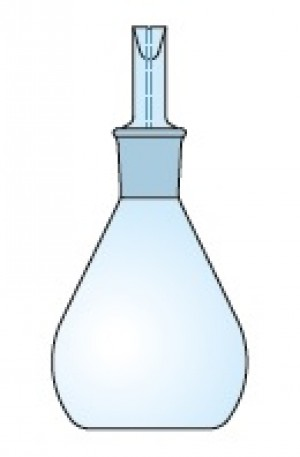
\includegraphics[width=0.30\linewidth]{imágenes/picnometro.jpg}

    \caption{Esquema de un picnómetro}
\end{figure}

Cabe destacar que aunque el volumen del picnómetro venga indicado en el aparato este valor es orientativo y se debe realizar el cálculo del volumen igual ya que, como se podrá observar posteriormente, el valor indicado y el valor real difieren un poco. Para el cálculo del volumen del picnómetro se pesará primero vacío y seco en la balanza y luego se realizarán diez medidas con el picnómetro lleno de agua. En las medidas del picnómetro con agua es importante llenarlo hasta desbordarlo y luego secarlo bien para que el volumen de líquido se mantenga constante siempre y no existan gotas de agua por fuera que interfieran en la medida.

\par Para calcular el volumen vamos a partir del concepto de densidad $(\rho = \frac{m}{V})$ y suponemos que el agua es un líquido de densidad conocida $(\rho_{o} = 1000 \: \frac{kg}{m^3}=1 \: \frac{g}{mL})$, para poder calcular así el volumen de agua que hay en el picnómetro con la siguiente relación:

\begin{equation}
    V = \frac{m-m_{p}}{\rho_{o}}
    \label{VolPicnometro}
\end{equation}

Donde $m$ es la media aritmética de los valores de la masa del picnómetro lleno de agua y $m_{p}$ es la masa del picnómetro vacío y seco.

\par Una vez calculado el volumen del picnómetro podemos empezar a determinar las densidades de diferentes materiales. En concreto, en esta práctica trabajamos con dos líquidos (Acetona y alcohol) y un sólido, el plomo.

\begin{itemize}
    \item Para el caso de los líquidos la metodología será muy parecida a las medidas realizadas con el agua. Llenaremos hasta desbordar el picnómetro con el líquido correspondiente, agua o alcohol, lo secaremos bien y pesaremos el picnómetro lleno. Repetiremos este proceso vaciándolo un poco y volviéndolo a llenar hasta tener diez medidas de la masa del picnómetro lleno con el líquido a estudiar. La ecuación de la densidad del líquido será la siguiente:
    
        \begin{equation}
            V=\frac{m'-m_{p}}{\rho}
            \label{VolLiquido}
        \end{equation}

    Igualando la Ec.\ref{VolPicnometro} con la Ec.\ref{VolLiquido} obtenemos la siguiente expresión para la densidad del líquido a estudiar:

        \begin{equation}
            \frac{m-m_{p}}{\rho_{o}}=\frac{m'-m_{p}}{\rho} \Rightarrow \frac{\rho}{\rho_{o}}=\frac{m'-m_{p}}{m-m_{p}}
            \label{Densidad liq}
        \end{equation}

        Donde $m'$ es la media aritmética de los valores de la masa del picnómetro con el líquido a estudiar, $m$ es la media aritmética de los valores de la masa del picnómetro lleno de agua y $m_{p}$ es la masa del picnómetro vacío y seco.

    \item Para medir la densidad de un sólido, en nuestro caso unos perdigones de plomo, lo primero que haremos es pesarlo seco antes de meterlo en el picnómetro. A continuación introducimos los perdigones en el picnómetro y lo llenamos con nuestro líquido de densidad conocida, el agua, y realizamos diez medidas vaciando un poco el picnómetro y volviéndolo a llenar.
    
    \begin{figure}[h!]
        \centering
        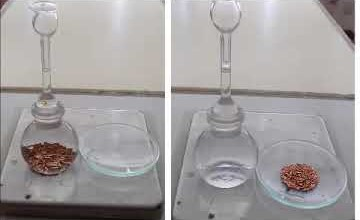
\includegraphics[width=0.50\linewidth]{imágenes/picnometriaSolido.jpg}
    
        \caption{Esquema de una picnometría de sólidos}
    \end{figure}

    Lo que tratamos de determinar con  estas medidas es la diferencia de masa entre el picnómetro lleno con solo agua y con agua y perdigones. La masa total del conjunto obedecerá la siguiente relación:
    
        \begin{equation}
            m_{T}=m_{P}+m_{s}+\rho_{o} \Delta V
            \label{RelacionMasas}
        \end{equation}
    
    Donde $\Delta V$ es el volumen del agua en el picnómetro con perdigones:

        \begin{equation}
            \Delta V = V_{P}-V_{s}=V_{P}-\frac{m_{s}}{\rho_{s}}
        \end{equation}

    Sustituyendo $\Delta V$ en la Ec.\ref{RelacionMasas} y despejando el volumen del picnómetro obtenemos:

    \begin{equation}
        V = \frac{m_{T}-m_{P}-m_{s}}{\rho_{o}}+\frac{m_{s}}{\rho_{s}}
    \end{equation}

    Igualando con la Ec.\ref{VolPicnometro} obtenemos:

    \begin{equation}
        \frac{\rho_{s}}{\rho_{o}}=\frac{m_{s}}{m_{s}+m-m_{T}}
        \label{Densidad Sólido}
    \end{equation}

    
\end{itemize}



\subsection{Viscosidad}

\begin{itemize}
    \item Viscosímetro
    \item Cronómetro
    \item Líquidos a estudiar
\end{itemize}

La segunda parte de la práctica consiste en un estudio de la viscosidad de diferentes líquidos, para los que calcularemos su coeficiente de viscosidad o viscosidad dinámica $(\eta )$. Este coeficiente se define como la fuerza por unidad de área necesaria para mantener un gradiente de velocidad unidad entre dos planos paralelos de un fluido situados a una distancia unidad. La viscosidad en el CGS (Sistema Cegesimal de Unidades, basado en el centímetro, el gramo y el segundo) es el \textbf{poise} $(g(cm\: s)^{-1})$. La otra magnitud empleada es la viscosidad cinemática, que se define como el cociente entre la viscosidad dinámica y la densidad del fluido. En el CGS se mide en \textbf{stokes} $(cm^2/s)$.

\par El coeficiente de viscosidad es inversamente proporcional a la velocidad de caída del líquido por un capilar, es decir cuánto más tarda el líquido en fluir por el capilar mayor será su viscosidad dinámica. Por tanto $\eta$ es directamente proporcional al tiempo empleado por el líquido en recorrer cierta distancia a lo largo del capilar y la fórmula que relaciona las magnitudes es la siguiente:

\begin{equation}
    \eta = k \cdot  \rho \cdot t
    \label{Viscosidad 1}
\end{equation}

Donde $\rho$ es la densidad del fluido. Para medir $\eta$ el procedimiento a seguir será medir el tiempo que tarda el fluido a estudiar en desplazarse entre las dos marcas de un viscosímetro como el de la Fig.\ref{Viscosímetro}.

\begin{figure}[h!]
    \centering
    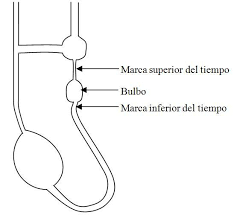
\includegraphics[width=0.4\linewidth]{imágenes/viscosimetro.png}

    \caption{Esquema de un viscosímetro}
    \label{Viscosímetro}
\end{figure}

No obstante el primer paso el conocer el valor de la constante de proporcionalidad $(k)$, independiente de cada capilar y, por tanto, independiente de cada viscosímetro. Para ello debemos trabajar con un líquido de densidad y viscosidad dinámica conocida, en nuestro caso será el agua a temperatura ambiente $T= 19,5\pm 0,5^{\circ} C$. Su coeficiente de viscosidad dinámica a la temperatura de trabajo se puede obtener a partir de la siguiente ecuación:

\begin{equation}
    \ln \frac{\eta}{\eta_{20}} = \frac{1,2348(20-T)-0,001467(T-20)^2}{T+96}
    \label{Coeficientes viscosidad}
\end{equation}

Donde $\eta_{20}$ es la viscosidad dinámica del agua a $20^{\circ}C$, que se toma como constante y tiene un valor de $0,01\: poise$.

\par Una vez conocido el valor de la viscosidad dinámica del agua a la temperatura de trabajo realizaremos diez medidas del tiempo que tarda el agua en fluir desde la marca superior hasta la marca inferior del viscosímetro. Cabe destacar que antes de realizar estas medidas se debe limpiar el viscosímetro por dentro minuciosamente, pues cualquier mota de polvo podría alterar considerablemente los tiempos medidos o incluso bloquear el agua y impedir que fluya por los capilares de forma normal.

\par Estas medidas nos servirán para determinar con mayor exactitud la constante del viscosímetro a partir de la Ec.\ref{Viscosidad 1} de la siguiente forma:

\begin{equation}
    k = \frac{\eta}{\rho \cdot t}
    \label{Coef Viscosimetro}
\end{equation}

Una vez determinada la constante del viscosímetro podemos proceder con rigor a determinar los diferentes coeficientes de viscosidad de los dos líquidos a estudiar: acetona y alcohol.

\newpage

\par El procedimiento a seguir con los dos líquidos es idéntico, vamos a medir el tiempo que tardan en fluir desde la marca superior hasta la marca inferior del viscosímetro, como se observa en la Fig.\ref{Viscosímetro}. En el caso de la acetona realizamos diez medidas de ese mismo tiempo, mientras que para el alcohol solo pudieron ser realizadas siete medidas por falta de tiempo. El cálculo de la viscosidad dinámica de cada líquido se realizará a partir de la Ec.\ref{Viscosidad 1}, con su respectiva incertidumbre obtenida a partir de propagación de incertidumbres.



\section{Análisis de datos}

\subsection{Densidad}

\subsubsection{Cálculo del volumen del picnómetro}

Como se explicó en la metodología, el primer paso de la práctica es calcular el volumen del picnómetro a partir de la Ec.\ref{VolPicnometro}. La masa del picnómetro vacío y seco es la siguiente:

\begin{equation}
    m_{p} = 19.12 \pm 0,01 \; g
\end{equation}

Donde la incertidumbre representa la precisión de la balanza empleada.

\par Para calcular el valor de la masa del picnómetro lleno de agua realizamos diez medidas y calculamos su media aritmética y su incertidumbre de tipo A y B con el siguiente tratamiento estadístico:

\begin{table}[h!]
    \centering
    \begin{tabular}{|c|c|}
    \hline
    Medida & $m \pm s(m)\; g$  \\ \hline
    $1$    & $45.74 \pm 0.01$ \\ \hline
    $2$    & $45.73 \pm 0.01$ \\ \hline
    $3$    & $45.76 \pm 0.01$ \\ \hline
    $4$    & $45.75 \pm 0.01$ \\ \hline
    $5$    & $45.78 \pm 0.01$ \\ \hline
    $6$    & $45.67 \pm 0.01$ \\ \hline
    $7$    & $45.66 \pm 0.01$ \\ \hline
    $8$    & $45.80 \pm 0.01$ \\ \hline
    $9$    & $45.78 \pm 0.01$ \\ \hline
    $10$   & $45.74 \pm 0.01$ \\ \hline
    \end{tabular}
    \caption{Medidas de la masa del picnómetro lleno de agua}
    \label{Pic Agua}
    \end{table}

\newpage

La media aritmética de la muestra inicial (Con $n=10$) y su desviación típica se calculan de la siguiente forma:

\begin{align}
    \overline{m} &= \frac{\sum_{i}^n m_{i}}{n} = 45.740 \; g 
    \label{Media1} \\
    s_{A}(m) &= \sqrt{\frac{\sum_{i}^n (m_i-\overline{m})^2}{n-1}} = 0.043 \; g
    \label{Desviación Típica de la muestra}
\end{align}

La desviación típica de la media se calcula de la siguiente forma:

\begin{equation}
    s_{A}(\overline{m}) = \frac{s_{A}(m)}{\sqrt{n}} = 0.014 \; g
    \label{Desv_T_agua}
\end{equation}


El siguiente paso será establecer los intervalos de confianza para eliminar los valores discordantes y tener datos con más precisión. Los intervalos vendrán determinados por la siguiente relación: $\overline{m} \pm k \cdot s_{A}(\overline{m})$, donde $k \cdot s_{A}(\overline{m})$ representa la incertidumbre expandida y $k$ es el factor de cobertura de la distribución T de Student. En todos los análisis posteriores tomaremos $k=2$ para obtener una probabilidad del $95 \%$.

\begin{align}
    \begin{split}
        \overline{m} - k \cdot s_{A}(m) \leq &m_{i} \leq \overline{m} + k \cdot s_{A}(m) \\
        45,654 \leq &m_{i} \leq 45.826
    \end{split}
\end{align}

A continuación debemos calcular el valor de la incertidumbre combinada de la muestra, que se calcula con la desviación típica de la media, calculada en la Ec.\ref{Desv_T_agua} y la incertidumbre de tipo B, que tomaremos como la precisión de la balanza, por lo que tendrá un valor de $0,01$:

\begin{equation}
    s_{C}(\overline{m}) = \sqrt{[s_{A}(\overline{m})]^2+[s_{B}(m)]^2} = 0,017 \; g
    \label{Inc combinada}
\end{equation}

Después de aplicar el factor de cobertura podemos observar que todos los datos experimentales se encuentran dentro del intervalo de confianza por lo que el valor final de la media de la masa del picnómetro con agua es el siguiente:

\begin{equation}
    \overline{m} = 45,740 \pm 0,017 \; g
\end{equation}

Por tanto, el volumen del picnómetro tomaría el siguiente valor, aplicando la Ec.\ref{VolPicnometro}:

\begin{equation}
    V = \frac{\overline{m}-m_{p}}{\rho_{o}}  = 26.621\; mL
\end{equation}

Para calcular la incertidumbre del volumen del picnómetro vamos a aplicar propagación de incertidumbres:

\begin{align}
    \begin{split}
    s(V) = &\sqrt{\left (\frac{\partial V}{\partial \overline{m}}\right )^2 s^2(\overline{m})  + \left (\frac{\partial V}{\partial m_{p}}\right )^2 s^2(m_{p})} \\
    s(V) = &\sqrt{\left (\frac{1}{\rho_{o}}\right )^2 s^2(\overline{m})  + \left (\frac{-1}{\rho_{o}}\right )^2 s^2(m_{p})} = 0.014 \; mL
    \end{split}
\end{align}

Por tanto, el valor final del volumen del picnómetro es el siguiente:

\begin{equation}
    V = 26,621 \pm 0,014 \; mL
\end{equation}

\subsubsection{Densidad de la acetona}

Una vez conocido el volumen del picnómetro podemos proceder a determinar las densidades de diferentes sustancias, en primer lugar la acetona. Como se explicó en la metodología, el primer paso será tomar diez medidas de la masa del picnómetro lleno de acetona:

\begin{table}[h!]
    \centering
    \begin{tabular}{|c|c|}
    \hline
    Medida & $m \pm s(m) \; g$\\ \hline
    $1$    & $40.38\pm 0,01$ \\ \hline
    $2$    & $40.43\pm 0,01$ \\ \hline
    $3$    & $40.39\pm 0,01$ \\ \hline
    $4$    & $40.34\pm 0,01$ \\ \hline
    $5$    & $40.34\pm 0,01$ \\ \hline
    $6$    & $40.35\pm 0,01$ \\ \hline
    $7$    & $40.33\pm 0,01$ \\ \hline
    $8$    & $40.30\pm 0,01$ \\ \hline
    $9$    & $40.28\pm 0,01$ \\ \hline
    $10$   & $40.29\pm 0,01$ \\ \hline
    \end{tabular}
    \caption{Medidas de la masa del picnómetro lleno de acetona}
    \label{Masas Acetona}
    \end{table}

A continuación debemos realizar un tratamiento estadístico similar al que hicimos con los datos de las masas del picnómetro lleno de agua. La media y la desviación típica de la muestra se calculan con las Ec.\ref{Media1} y Ec.\ref{Desviación Típica de la muestra} respectivamente:

\begin{align}
    \overline{m}_{ac} = &40.343 \; g    \\
    s_{A}(m_{ac}) &= 0.045 \; g
\end{align}

Aplicando el factor de cobertura $k=2$ obtenemos el intervalo de confianza $[40,253 \; g ; 40,433 \; g]$, que engloba a todos nuestros datos. El siguiente paso será calcular la incertidumbre combinada (Usando la Ec.\ref{Inc combinada}) a partir de la desviación típica de la media (Usando la Ec.\ref{Desv_T_agua}) y la incertidumbre de tipo B, que tomaremos otra vez como $0,01$, el valor de la precisión de la balanza:

\begin{align}
    &s_{A}(\overline{m}_{ac}) = 0.014 \; g \\
    s_{C}(\overline{m}_{ac}) = &\sqrt{0,014^2 + 0,01^2} = 0.017 \; g
\end{align}

Por tanto, el valor final de la media de la masas del picnómetro lleno de acetona es el siguiente:

\begin{equation}
    \overline{m}_{ac} = 40,343 \pm 0,017 \; g
\end{equation}

Este valor nos servirá para calcular la densidad de la acetona a partir de la Ec.\ref{Densidad liq}:

\begin{equation}
    \frac{\rho}{\rho_o}=\frac{\overline{m}_{ac}-m_{p}}{\overline{m}-m_{p}} \Rightarrow \rho_{ac} = \frac{40,34-19,12}{45,74-19,12} = 0.79723 \; \frac{g}{cm^3}
\end{equation}

Aplicando propagación de incertidumbres podemos calcular la incertidumbre de esta medida indirecta:

\begin{gather}
    s(\rho_{ac}) = \sqrt{\left (\frac{\partial \rho_{ac}}{\partial \overline{m}_{ac}} \right )^2 s^2(\overline{m}_{ac})  +  \left (\frac{\partial \rho_{ac}}{\partial \overline{m}} \right )^2 s^2(\overline{m})  +  \left (\frac{\partial \rho_{ac}}{\partial m_{p}} \right )^2 s^2(m_{p})} \\
    s(\rho_{ac}) = \sqrt{\left (\frac{1}{\overline{m}-m_{p}} \right )^2 s^2(\overline{m}_{ac})  +  \left (\frac{-(\overline{m}_{ac}-m_{p})}{(\overline{m}-m_{p})^2} \right )^2 s^2(\overline{m})  +  \left (\frac{\overline{m}_{ac}-\overline{m}}{(\overline{m}-m_{p})^2} \right )^2 s^2(m_{p})} \nonumber  \\
    s(\rho_{ac}) = 0.00083 \; \frac{g}{cm^3} \nonumber
    \label{Inceridumbre densidad liq}
\end{gather}

Por tanto el valor final de la densidad de la acetona es:

\begin{equation}
    \rho_{ac} = 0.79723 \pm 0.00083 \; \frac{g}{cm^3}
\end{equation}

El valor real de la densidad de la acetona es de $0,784 \; \frac{g}{cm^3}$, que se encuentra bastante próximo al resultado experimental pero no entra dentro del rango de incertidumbre. Los valores de la masa del picnómetro con acetona presentan muy poca dispersión por lo que el motivo de discordancia es otro.La diferencia entre los dos valores se puede explicar probablemente por la presencia de cierta cantidad de agua en el picnómetro, sustancia de una densidad mayor que la de la acetona y que, de estar presente, aumentaría el valor experimental de la densidad. 

\newpage

\subsubsection{Densidad del alcohol}

Para determinar la densidad del alcohol procederemos igual que con la acetona. En primer lugar, las diez medidas de la masa del picnómetro lleno de alcohol son las siguientes:

\begin{table}[h!]
    \centering
    \begin{tabular}{|c|c|}
    \hline
    Medida & $m \pm s(m) \: g$   \\ \hline
    $1$    & $41.12\pm0.01$ \\ \hline
    $2$    & $41.13\pm0.01$ \\ \hline
    $3$    & $41.13\pm0.01$ \\ \hline
    $4$    & $41.12\pm0.01$ \\ \hline
    $5$    & $41.13\pm0.01$ \\ \hline
    $6$    & $41.11\pm0.01$ \\ \hline
    $7$    & $41.02\pm0.01$ \\ \hline
    $8$    & $41.07\pm0.01$ \\ \hline
    $9$    & $41.11\pm0.01$ \\ \hline
    $10$   & $41.11\pm0.01$ \\ \hline
    \end{tabular}
    \caption{Medidas de la masa del picnómetro lleno de alcohol}
    \label{Masas Alcohol}
    \end{table}

A partir de un tratamiento estadístico idéntico al que realizamos con la acetona obtuvimos el siguiente dato de incertidumbre y la media de las masas:

\begin{gather}
    \overline{m}_{al} = 41.105 \; g \\
    s_{A}(m_{al}) =  0.033 \; g 
\end{gather}

Si aplicamos el factor de cobertura $k=2$ obtenemos el intervalo de confianza $[41.039 \; g ; 41.171 \; g]$, que nos obliga a dejar fuera a la medida número 7, de $41,02 \;g$. Con estos datos podemos calcular ya la nueva media, la desviación típica de la media y la incertidumbre combinada de forma análoga a como lo hicimos con la acetona.

\begin{gather}
    \overline{m}_{al} = 41.1144 \; g\\
    s_{A}(\overline{m}_{al}) = 0.0059 \; g\\
    s_{C}(\overline{m}_{al}) = 0.012 \; g
\end{gather}

El valor final de la media de las masas del picnómetro lleno de alcohol es:

\begin{equation}
    \overline{m}_{al} = 41,114 \pm 0,012 \; g
\end{equation}

Sustituyendo este valor en la Ec.\ref{Densidad liq} podemos obtener el valor de la densidad del alcohol:

\begin{equation}
    \rho_{al}  = 0.82620 \; \frac{g}{cm^3}
\end{equation}

Por último, calcularemos la incertidumbre de la densidad del alcohol aplicando la Ec.\ref{Inceridumbre densidad liq}, sustituyendo, por supuesto, la media de las masas de la acetona por la del alcohol. De esta forma el valor final de la densidad del alcohol es:

\begin{equation}
    \rho_{al} = 0.82620 \pm 0.00069 \; \frac{g}{cm^3}
\end{equation}

El alcohol empleado en la práctica fue alcohol etílico o etanol, cuya densidad real es de $0,789 \frac{g}{cm^3}$. Este valor se encuentra también bastante próximo al experimental pero se sale del rango de incertidumbre. Esta discordancia se puede explicar de la misma forma que la anterior, la presencia de cierta cantidad agua en el picnómetro (Líquido de densidad mayor que la del alcohol) aumenta ligeramente el valor experimental de la densidad del alcohol. Como podemos observar, el ligero aumento de la densidad experimental se repite con ambos líquidos, lo que refuerza nuestras suposiciones de que la presencia de cierta cantidad de agua (Algo difícil de evitar) pueda estar causando estas variaciones.


\subsubsection{Densidad de un sólido: El plomo}

Para determinar la densidad del plomo lo primero que hicimos fue pesar nuestros perdigones de plomo:

\begin{equation}
    m_{pe} = 9,61 \pm 0,01 \; g
\end{equation}

A continuación realizamos diez medidas de la masa del picnómetro con los perdigones lleno de agua, nuestro líquido de densidad conocida:

\newpage

\begin{table}[h!]
    \centering
    \begin{tabular}{|c|c|}
    \hline
    Medida & $m \pm s(m) \; g$ \\ \hline
    $1$    & $54.42\pm0.01$ \\ \hline
    $2$    & $54.43\pm0.01$ \\ \hline
    $3$    & $54.49\pm0.01$ \\ \hline
    $4$    & $54.44\pm0.01$ \\ \hline
    $5$    & $54.49\pm0.01$ \\ \hline
    $6$    & $54.51\pm0.01$ \\ \hline
    $7$    & $54.40\pm0.01$ \\ \hline
    $8$    & $54.40\pm0.01$ \\ \hline
    $9$    & $54.46\pm0.01$ \\ \hline
    $10$   & $54.46\pm0.01$ \\ \hline
    \end{tabular}
    \caption{Medidas de la masa del picnómetro lleno de agua con los perdigones}
    \label{Masas Perdigones}
    \end{table}

El tratamiento estadístico a realizar es el mismo que en apartados anteriores:

\begin{gather}
    \overline{m}_{T} = 54.450 \; g \\
    s_{A}(m_{T}) = 0.037 \; g
\end{gather}

Aplicando el factor de cobertura $k=2$ obtenemos el intervalo $[54,376 \; g  ; 54,524 \; g]$, dentro del que se encuentran todos nuestros datos. Por tanto, podemos calcular la desviación típica de la media y la incertidumbre combinada, incluyendo la incertidumbre de tipo B, que será igual que en otros apartados $0,01$.

\begin{gather}
    s_{A}(\overline{m}_{T}) = 0.012 \; g \\
    s_{C}(\overline{m}_{T}) = 0.015 \; g
\end{gather}



Por tanto, la media de las masas del picnómetro con perdigones y agua es la siguiente:

\begin{equation}
    \overline{m}_{T}=54,450 \pm 0,015 \; g
\end{equation}

Este valor nos servirá para calcular la densidad del plomo a partir de la Ec.\ref{Densidad Sólido}

\begin{equation}
    \frac{\rho_{s}}{\rho_{o}}=\frac{m_{s}}{m_{s}+m-m_{T}} \Rightarrow \rho_{Pb} = \frac{m_{pe}}{m_{pe}+\overline{m}-\overline{m}_{T}} = 10.6659\;  \frac{g}{cm^3}
\end{equation}

Aplicando propagación de incertidumbres podemos calcular el valor de la incertidumbre de la densidad:

\begin{gather}
    s(\rho_{Pb}) = \sqrt{\left (\frac{\partial \rho_{Pb}}{\partial m_{pe}} \right )^2 s^2(m_{pe})  +  \left (\frac{\partial \rho_{Pb}}{\partial \overline{m}} \right )^2 s^2(\overline{m})  +  \left (\frac{\partial \rho_{Pb}}{\partial \overline{m}_{T}} \right )^2 s^2(\overline{m}_{T})} \\ \textstyle
    s(\rho_{ac}) =
    \sqrt{\left (\frac{\overline{m}-\overline{m}_{T}}{(\overline{m}+m_{pe}-\overline{m}_{T})^2} \right )^2 s^2(m_{pe})  +  \left (\frac{-m_{pe}}{(\overline{m}+m_{pe}-\overline{m}_{T})^2} \right )^2 s^2(\overline{m})  +  \left (\frac{\overline{m}-\overline{m}_{T}}{(\overline{m}+m_{pe}-\overline{m}_{T})^2} \right )^2 s^2(m_{T})}\nonumber  \\
    s(\rho_{ac}) = 0.0043 \; \frac{g}{cm^3} \nonumber
\end{gather}

Por tanto el valor de la densidad del plomo es de:

\begin{equation}
    \rho_{Pb} = 10.6659 \pm 0.0043 \; \frac{g}{cm^3}
\end{equation}

El valor real de la densidad del plomo es de $11.35 \; \frac{g}{cm^3}$, que se aleja un poco del valor experimental, algo más de media unidad. La aplicación del factor de cobertura nos llevó a que trabajamos con una buena precisión, quizás el fallo se debe a la poca exactitud de los datos. Una posibilidad bastante razonable es que los perdigones no sean integramente de plomo, sino de alguna aleación que altere su densidad.


\subsection{Viscosidad}

\subsubsection{Cálculo de la constante del viscosímetro}

A partir de la Ec.\ref{Coeficientes viscosidad} podemos determinar el valor de la viscosidad dinámica a la temperatura de trabajo despejándola de esta forma:

\begin{align}
    \begin{split}   %El split ayuda a poner solo un número
    \eta_{ag} &= \eta_{20}\: e^{\frac{1,2348(20-T)-0,001467(T-20)^2}{T+96}} \\
    \eta_{ag} &= 0.010054 \: poise
    \end{split}
\end{align}

La incertidumbre obtenida para la viscosidad dinámica del agua a la temperatura de trabajo obtenida a partir de propagación de incertidumbres es la siguiente:

\begin{align}
    \begin{split}
    s(\eta_{ag}) &= \sqrt{\left (\frac{\partial \eta_{ag}}{\partial T}\right )^2 s^2(T)} \\
    s(\eta_{ag}) &= 0,000054 \:poise
    \end{split}
\end{align}

Por tanto, el valor de la constante de viscosidad del agua a la temperatura de trabajo es el siguiente:

\begin{equation}
    0,010054 \pm 0,000054 \: poise
\end{equation}

Como se explicó en el apartado anterior, una vez conocida la viscosidad dinámica del agua a la temperatura de trabajo vamos a calcular la constante del viscosimétro. Para ello las medidas obtenidas fueron las siguientes:

\begin{table}[h!]
    \centering
    \begin{tabular}{|c|c|}
    \hline
    Medida & $T \; (s)$\\ \hline
    $1$    & $153.45$ \\ \hline
    $2$    & $156.20$ \\ \hline
    $3$    & $154.89$ \\ \hline
    $4$    & $154.54$ \\ \hline
    $5$    & $153.50$ \\ \hline
    $6$    & $154.06$ \\ \hline
    $7$    & $154.01$ \\ \hline
    $8$    & $154.27$ \\ \hline
    $9$    & $154.64$ \\ \hline
    $10$   & $154.10$ \\ \hline
    \end{tabular}
    \caption{Medidas del tiempo de flujo del agua}
    \label{Tiempos agua}
    \end{table}

    \par La incertidumbre de estos valores vendrá dada por el tiempo medio de reacción de un humano ante un estímulo visual, igual que en el apartado anterior:

    \begin{equation}
        s(T) = 0,25 \; s
    \end{equation}    

    A continuación, vamos a aplicar ciertas técnicas estadísticas para calcular la media del tiempo con su incertidumbre. En primer lugar debemos calcular la media y la desviación típica de la muestra:

    \begin{equation}
        \begin{gathered}
            \overline{T} = 154.36 \; s \\
            s_A (T) = 0.75 \; s
        \end{gathered}
    \end{equation}
    
    Ahora construiremos nuestro intervalo de confianza aplicando el factor de cobertura $k=2$. En este caso obtuvimos el intervalo $[152,86\; s;155,86\; s]$. Este intervalo deja fuera al dato $T=156,20 \; s$, por lo que deberemos calcular otra vez la media y la desviación típica de la muestra:
    
    \begin{equation}
        \begin{gathered}
            \overline{T} = 154.16 \; s \\
            s_A (T) = 0.46 \; s
        \end{gathered}
    \end{equation}
    
    A partir de estos valores calcularemos la desviación típica de la media y la incertidumbre combinada, con la que expresaremos el resultado:
    
    \begin{equation}
        \begin{gathered}
            s_A(\overline{T}) = 0.15 \; s \\
            s_C(\overline{T}) = 0.29 \; s
        \end{gathered}
    \end{equation}
    
Por tanto el valor de referencia que usaremos para el tiempo de caída fue de:
    
\begin{equation}
    T = 154.16 \pm 0.29 \; s
\end{equation}

A continuación calcularemos el valor de la constante del viscosímetro con su incertidumbre aplicando la Ec.\ref{Coef Viscosimetro}:

\begin{equation}
    k = 6.522 \cdot 10^{-5 }\pm 3.7 \cdot 10^{-7} \; \frac{poise\cdot cm^3}{g\cdot s}
\end{equation}

La incertidumbre la calculamos a partir de propagación de incertidumbres, como se detallará a continuación. Para el cálculo de esta incertidumbre supusimos una densidad del agua constante con un valor de $1 \; g\cdot cm^{-3}$:

\begin{equation}
    \begin{gathered}
        s(k) = \sqrt{\left (\frac{\partial k}{\partial \eta }\right )^2 s^2(\eta) + \left (\frac{\partial k}{\partial t}\right )^2s^2(t)} = \sqrt{\left (\frac{1}{t}\right )^2s^2(\eta) + \left (\frac{-\eta}{t^2}\right )^2s^2(t)} \\ s(k) = 3.7 \cdot 10^{-7} \; \frac{poise\cdot cm^3}{g\cdot s}
    \end{gathered}
\end{equation}

\subsubsection{Viscosidad de la acetona}

El procedimiento para determinar la viscosidad de la acetona va a ser similar al empleado en el apartado anterior, solo que ahora una vez conocida la constante del viscosímetro aplicaremos la Ec.\ref{Viscosidad 1} para calcular la viscosidad dinámica de la acetona.

\par En primer lugar necesitamos un valor de referencia para el tiempo de flujo, que obtendremos de aplicar el mismo tratamiento estadístico realizado anteriormente a los valores del tiempo de flujo medidos en el laboratorio, reflejados en la siguiente tabla:

\begin{table}[h!]
    \centering
    \begin{tabular}{|c|c|}
    \hline
    Medida   & $T \; (s)$ \\ \hline
    1  & 69,51 \\ \hline
    2  & 69,99 \\ \hline
    3  & 69,58 \\ \hline
    4  & 69,8  \\ \hline
    5  & 69,85 \\ \hline
    6  & 69,73 \\ \hline
    7  & 69,84 \\ \hline
    8  & 69,67 \\ \hline
    9  & 69,59 \\ \hline
    10 & 69,80  \\ \hline
    \end{tabular}
    \caption{Medidas del tiempo de flujo de la acetona}
    \label{T acetona}
\end{table}

\newpage

La incertidumbre de estos valores vendrá dada por el tiempo medio de reacción de un humano ante un estímulo visual, igual que en el apartado anterior:

\begin{equation}
    s(T) = 0,25 \; s
\end{equation}

En primer lugar debemos calcular la media y la desviación típica de la muestra:

\begin{equation}
    \begin{gathered}
        \overline{T} = 69.74 \;s\\
        s_A(T) = 0.14 \;s
    \end{gathered}
\end{equation}

El siguiente paso es aplicar el factor de cobertura $k=2$ para obtener nuestro intervalo de confianza, en este caso $[69,46\; s;70,02\; s]$. Todos los datos medidos entran dentro del intervalo de confianza por lo que no hay que descartar ninguno. La desviación típica de la media y la incertidumbre combinada tienen los siguientes valores:

\begin{equation}
    \begin{gathered}
        s_A(\overline{T}) = 0.044 \; s \\
        s_C(\overline{T}) = 0.25 \; s
    \end{gathered}
\end{equation}

Por tanto el valor final del tiempo de flujo con su incertidumbre es:

\begin{equation}
    T_{ac} = 69.74 \pm 0.25 \; s
\end{equation}

Finalmente, aplicando la Ec.\ref{Viscosidad 1} podemos calcular la viscosidad dinámica de la acetona:

\begin{equation}
    \eta_{ac} = 0.003626 \; poise
\end{equation}

La incertidumbre de la viscosidad dinámica la calcularemos aplicando propagación de incertidumbres a la Ec.\ref{Viscosidad 1}:

\begin{equation}
    \begin{gathered}
    s\left(\eta_{ac}\right) =\sqrt{\left(\frac{\partial \eta_{ac}}{\partial k}\right)^2 s^2(k)+\left(\frac{\partial \eta_{a c}}{\partial \rho_{a c}}\right)^2 s^2\left(\rho_{ac}\right)+\left(\frac{\partial \eta_{ac}}{\partial T_{ac}}\right)^2 s^2\left(T_{a c}\right)} \\
    s\left(\eta_{a c}\right)  =\sqrt{\left(\rho_{a c} \cdot T_{a c}\right)^2 s^2(k)+\left(k \cdot T_{a c}\right)^2 s^2\left(\rho_{a c}\right)+\left(\rho_{a c} \cdot k\right)^2 s^2\left(T_{a c}\right)} \\
    s(\eta_{ac}) = 2,5 \cdot 10^{-5} \; poise
    \end{gathered}
    \label{Inc visc}
\end{equation}

Por tanto, el valor final de la viscosidad de la acetona es:

\begin{equation}
    \eta_{ac} = 0.003626 \pm 2,5 \cdot 10^{-5} \; poise
\end{equation}

El valor real de la viscosidad de la acetona a $20^{\circ} C$ es de $0,0032 \; poise$, que se acerca bastante al valor medido experimentalmente, aunque no entra dentro del intervalo de incertidumbre.


\subsubsection{Viscosidad del alcohol}

El procedimiento con el alcohol va a ser análogo al realizado con la acetona. Los datos del tiempo de flujo medidos figurarán en la siguiente tabla:

\begin{table}[h!]
    \centering
    \begin{tabular}{|c|c|}
    \hline
    Medida  & $T \;(s)$ \\ \hline
    1 & 312,88 \\ \hline
    2 & 315,22 \\ \hline
    3 & 314,57 \\ \hline
    4 & 314,47 \\ \hline
    5 & 315,96 \\ \hline
    6 & 315,74 \\ \hline
    7 & 313,51 \\ \hline
    \end{tabular}
    \caption{Datos del tiempo de flujo del alcohol}
    \label{T alcohol}
    \end{table}

Cabe destacar que para el tiempo de flujo del alcohol solo contamos con 7 medidas, pues no pudimos realizar las diez por falta de tiempo, como mencionamos anteriormente.

\par La incertidumbre de estos valores vendrá dada por el tiempo medio de reacción de un humano ante un estímulo visual, igual que en el apartado anterior:

\begin{equation}
    s(T) = 0,25 \; s
\end{equation}    

Para determinar un valor de referencia del tiempo de flujo vamos a aplicar el mismo tratamiento estadístico que anteriormente. La media y la desviación típica de la muestra son:

\begin{equation}
    \begin{gathered}
        \overline{T} = 314.6\; s\\
        s_A(T) =  1.0 \; s
    \end{gathered}
\end{equation}

Aplicando el factor de cobertura $k=2$ obtenemos un intervalo de confianza de $[312,6 \;s;316,6\; s]$, dentro del que se encuentran todos los datos medidos. Por tanto no tenemos que descartar ningún dato y podemos proceder a calcular la desviación típica de la media y la incertidumbre combinada:

\begin{equation}
    \begin{gathered}
        s_A(\overline{T}) = 0.40 \; s \\
        s_C(\overline{T}) = 0.47 \; s
    \end{gathered}
\end{equation}

Por tanto, el valor de referencia del tiempo de flujo para el alcohol es:

\begin{equation}
    T = 314.6 \pm 0.47 \; s
\end{equation}

Aplicando las Ec.\ref{Viscosidad 1} y Ec.\ref{Inc visc} (Sustituyendo los valores relativos al alcohol) obtenemos el siguiente valor para la viscosidad dinámica del alcohol y su incertidumbre:

\begin{equation}
    \eta_{al} =  0.01695 \pm 0.00010 \; poise
\end{equation}

El valor teórico de la viscosidad del alcohol es de $0,012 \; poise$, que, aún sin entrar dentro del intervalo de incertidumbre, se acerca bastante a nuestro valor experimental.

\newpage

\section{Conclusión}

Como conclusión vamos a realizar una exposición de todos los resultados obtenidos, para poder analizar los resultados de forma global. La primera parte de la práctica se centraba en el concepto de densidad de diferentes materiales, dos líquidos y un sólido. Los resultados obtenidos (Comparados con el valor real) fueron los siguientes:


\begin{table}[h!]
    \centering
    \begin{tabular}{|c|c|c|}
        \hline
        Material & $\rho  \; (g \cdot cm^{-3})$ & $\rho _E\pm s(\rho_E) \; (g \cdot cm^{-3})$ \\ \hline
        Acetona &$0, 784$ & $0,79723 \pm 0,00083$ \\ \hline
        Alcohol & $0, 789$ & $0,82620 \pm  0,00069$\\ \hline
        Plomo & $11,35$ & $10,6659 \pm 0,0043$ \\ \hline
    \end{tabular}
    \caption{Densidades reales y resultados experimentales}
\end{table}

Donde $\rho$ representa la densidad real y $\rho_E$ representa la densidad determinada experimentalmente. Como podemos observar las densidades experimentales de los líquidos se acercan considerablemente al valor real y la densidad del plomo, aunque difiere algo más, también entra dentro de un margen razonable, sobre todo considerando que los perdigones empleados probablemente no estuvieran hechos enteramente de plomo. Por tanto podemos concluír que en esta primera parte de la práctica los resultados fueron satisfactorios.

\par En la segunda parte de la práctica el objetivo fue determinar la viscosidad dinámica de los dos líquidos con los que trabajamos antes, la acetona y el alcohol. Los resultados obtenidos fueron los siguientes:

\begin{table}[h!]
    \centering
    \begin{tabular}{|c|c|c|}
        \hline
        Material & $\eta \; (poise)$ & $\eta_E \pm s(\eta_E) \; (poise)$ \\ \hline
        Acetona & $0,0032$ & $0,003626 \pm 0,000025$ \\ \hline
        Alcohol &$0,012$ & $0,01695 \pm  0,00010$\\ \hline
    \end{tabular}
\end{table}

Los resultados obtenidos reflejan de una forma bastante fiel los valores reales de la viscosidad dinámica de ambos líquidos, a pesar de las pequeñas diferencias. Una de las posibles explicaciones para estas diferencias es el cambio de temperatura, pues la viscosidad, que es una medida de la resistencia del líquido a fluir, tiene cierta dependencia de la temperatura. Esta dependencia tiene su origen a escala molecular, cuando la temperatura aumenta, y con ello la energía térmica de las partículas, se reducen las fuerzas intermoleculares que ejercen entre sí las partículas, disminuyendo su viscosidad. En la siguiente gráfica podemos ver una representación de la viscosidad de varios líquidos, en este caso estática (Medida en $cSt$), en función de la temperatura:

\begin{figure}[h!]
    \centering
    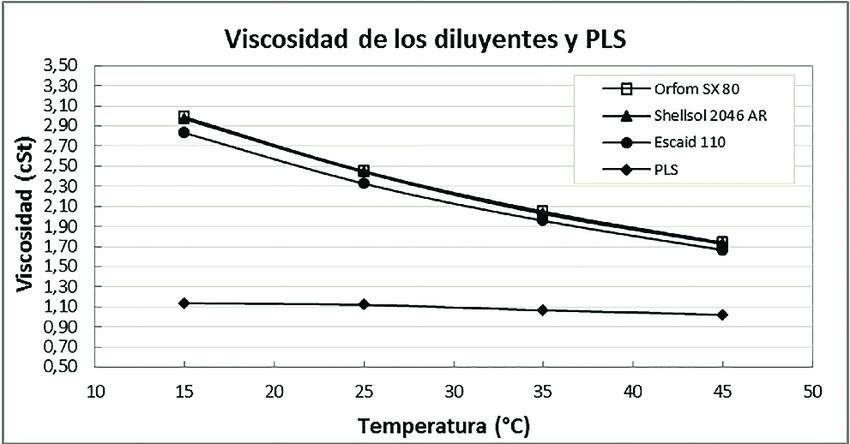
\includegraphics[width=0.65\linewidth]{imágenes/viscosidadT.png}
    \caption{Viscosidad estática de varios líquidos en función de su temperatura}
\end{figure}

\newpage

Los valores de referencia de la viscosidad que aparecen en la tabla son los valores medidos a una temperatura de $20^{\circ}C$ y una presión de $ 1 \;atm$. Aunque no contamos con los datos de la temperatura de nuestro laboratorio,previsiblemente se encontraba por debajo de esos $20^{\circ}C$, por lo que es una explicación bastante razonable para que el valor de la viscosidad medido sea mayor que el real. 

\par Otra posible explicación es que el conducto del viscosímetro no estuviera suficientemente limpio, quedando alguna mota de polvo dentro de él que dificultara el flujo de los líquidos, aumentando así su viscosidad.

\par Finalmente, pese a estas pequeñas discordancias en general los resultados de las medidas se correspondían bastante con la realidad, por lo que podemos afirmar que hemos alcanzado los objetivos de la práctica. Además de eso, hemos adquirido experiencia en el manejo de aparatos como el picnómetro o el viscosímetro.

\chapter{Muelle}

\section{Introducción teórica}

El objetivo principal de esta práctica es estudiar el comportamiento de un muelle ante distintas situaciones así como su aplicación a la hora de calcular densidades de diferentes materiales, tanto sólidos como líquidos. El fundamento teórico principal de esta práctica es la ley de Hooke, que establece una relación entre la fuerzaque ejerce el muelle cuando sufre una deformación:

\begin{equation}
    F = -k\Delta x
\end{equation}

Donde $k$ es la constante elástica del muelle y $\Delta x$ es la deformación. El signo negativo indica que es una fuerza de recuperación, se opone siempre a la deformación, intentando devolver el muelle a su posición de equilibrio. No obstante, la ley de Hooke no es válida para todas las situaciones, el muelle cuenta con un límite elástico que si lo sobrepasamos provocaremos que no pueda volver a la posición de retorno.

\par Para la realización de esta práctica vamos a suponer un muelle de masa despreciable del que cuelga una masa $m$. El diagrama de fuerzas se puede observar en la Fig.\ref{Diagrama fuerzas}.

\newpage

\begin{wrapfigure}{r}{0.35\textwidth}
    \centering
    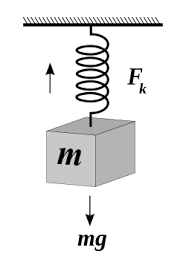
\includegraphics[width=0.75\linewidth]{Images/fuerzas hooke.png}
    \caption{Diagrama de fuerzas inicial}
    \label{Diagrama fuerzas}
\end{wrapfigure}

Cuando el sistema alcanza el equilibrio después de colgar la masa tenemos la siguiente relación:

\begin{equation}
    mg = k\Delta x
    \label{Met estatico}
\end{equation}

Cuando se provoca una nueva deformación el sistema abandona el equilibrio y comienza a oscilar siguiendo un M.A.S. El movimiento ondulatorio se puede modelizar a partir de la ecuación de su posición, que nos permite conocer su velocidad y su aceleración derivando:

\begin{equation}
    \left\{ \begin{array}{l}
        x(t) = A \cos (\varphi - \omega t) \\
        v(t) = \frac{dx}{dt} = -A \omega \sin (\varphi - \omega t) \\
        a(t) = \frac{d^2x}{dt^2} = -A \omega^2 \cos (\varphi - \omega t)
        \end{array}
    \right.
\end{equation}

A partir de estas ecuaciones podemos conocer la aceleración en función de la posición y de la velocidad angular. Si relacionamos por medio de la 2ª ley de Newton la fuerza (Ley de Hooke), con la aceleración obtenemos la siguiente relación:

\begin{equation}
    \begin{gathered}
    a = -\omega^2 x \Rightarrow m\overbrace{(-\omega^2x)}^a = \overbrace{-kx}^F \Rightarrow \omega = \sqrt{\frac{k}{m}} \\
    \omega = \frac{2\pi}{T} \Rightarrow T= 2\pi \sqrt{\frac{m}{k}}
    \end{gathered}
    \label{Met dinamico}
\end{equation}

Donde $T$ representa el período de oscilación del muelle.

\par A partir de estas relaciones podemos calcular la constante elástica del muelle de dos formas diferentes, por el método estático o por el método dinámico. El método estático se basa en la Ec.\ref{Met estatico}, midiendo la deformación que provoca una determinada masa. Por otra parte, el método dinámico se basa en la Ec.\ref{Met dinamico}, midiendo los diferentes períodos de oscilación que provocan diferentes masas. El objetivo de la primera parte de la práctica será determinar la constante elástica $k$ de un muelle a partir de estos dos métodos.

\par En la segunda parte de la práctica abordaremos las aplicaciones de un muelle para la determinación de la densidad de diferentes materiales (Sólidos y líquidos). Partiremos de la posición de equilibrio del muelle con una masa $m$ colgando, como en la Fig.\ref{Diagrama fuerzas}. El fundamento teórico de esta parte será la combinación del principio de Arquímedes con la ley de Hooke. El principio de Arquímedes nos afirma que si sumergimos un cuerpo total o parcialmente en un líquido este sufrirá un empuje hacia arriba igual al peso del fluido desalojado. Por tanto, si sumergimos nuestra masa $m$ en un líquido esta sufrirá un empuje vertical y alcanzará una nueva posición de equilibrio con una deformación menor. Las fuerzas que actúan sobre la masa $m$ en esta nueva situación de equilibrio son:

\begin{equation}
    \sum \vec{F} = 0 \Rightarrow \vec{P} + \vec{F}_k + \vec{E} = 0
\end{equation}

Donde $\vec{P}$ es el peso, $\vec{F}_k$ es la fuerza de recuperación y $\vec{E}$ es el empuje que ejerce el líquido. Si trabajamos con los módulos de las fuerzas y expresamos las masas en función de la densidad ($\rho = \frac{m}{V}$) tenemos que:

\begin{equation}
    \overbrace{\rho_s V_s g}^{\vec{P}} = \overbrace{\rho_L V_s g}^{\vec{E}} + \overbrace{k \Delta x'}^{\vec{F}_k} \Rightarrow \rho_s V_s g - \rho_L V_s g = k\Delta x'
\end{equation}

Si restamos esta ecuación a la Ec.\ref{Met estatico} expresada en función de la densidad ($\rho_s V_s g = k\Delta x$) obtenemos que:

\begin{equation}
    \rho_L V_s g = k (\Delta x -\Delta x')
    \label{Relacion sol liquido}
\end{equation}

Si dividimos la Ec.\ref{Met estatico} en función de la masa entre la Ec.\ref{Relacion sol liquido} obtenemos que:

\begin{equation}
    \rho_s = \rho_L \frac{\Delta x}{\Delta x - \Delta x'}
    \label{Densidad sol}
\end{equation}

Para la determinación de la densidad del líquido solo tendríamos que despejar su valor de la ecuación anterior:

\begin{equation}
    \rho_L = \rho_s \frac{\Delta x- \Delta x'}{\Delta x}
    \label{Densidad liq}
\end{equation}

En la última parte de la práctica trataremos de determinar el valor de la gravedad mediante la caída libre de un objeto.

\begin{figure}[h!]
    \centering
    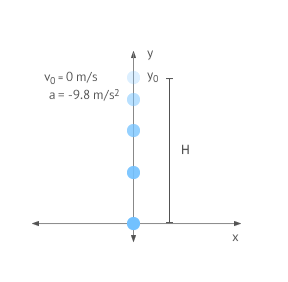
\includegraphics[width=0.5\linewidth]{Images/caidalibre.png}
    \caption{Caída libre ideal de un cuerpo}
\end{figure}

\newpage

Para ello partiremos de un objeto al que someteremos a una caída libre ideal, despreciando el efecto del rozamiento que ejerce el aire. Un cuerpo en una caída libre ideal sigue un MRUA en el eje $Y$ que se puede modelizar fácilmente con la siguiente ecuación:

\begin{equation}
    y = y_0 +v_0t +\frac{1}{2} at^2 \Rightarrow y = h -\frac{1}{2}gt^2 \overbrace{\Rightarrow}^{y=0} t = \sqrt{\frac{2h}{g}}
    \label{Formula C.L}
\end{equation}

\newpage

\section{Materiales y metodología}

\subsection{Determinación de la constante elástica de un muelle}

En la primera parte de la práctica determinaremos el valor de la constante elástica de nuestro muelle mediante los dos métodos antes descritos, el método estático y el método dinámico. En el método estático mediremos la relación entre la fuerza que soporta el muelle y su deformación mientras que en el método dinámico mediremos la relación entre la masa que cuelga del muelle y su período. Los materiales empleados para ambas mediciones fueron los siguientes:

\begin{itemize}
    \item Muelle pendurado de un soporte
    \item Pesas de diferentes calibres colgadas de un portapesas
    \item Balanza para medir la masa de las diferentes pesas
    \item Regla vertical para medir la deformación, empleada en el método estático
    \item Cronómetro, empleado para medir el período en el método dinámico
\end{itemize}

\begin{wrapfigure}{r}{0.4\textwidth}
    \centering
    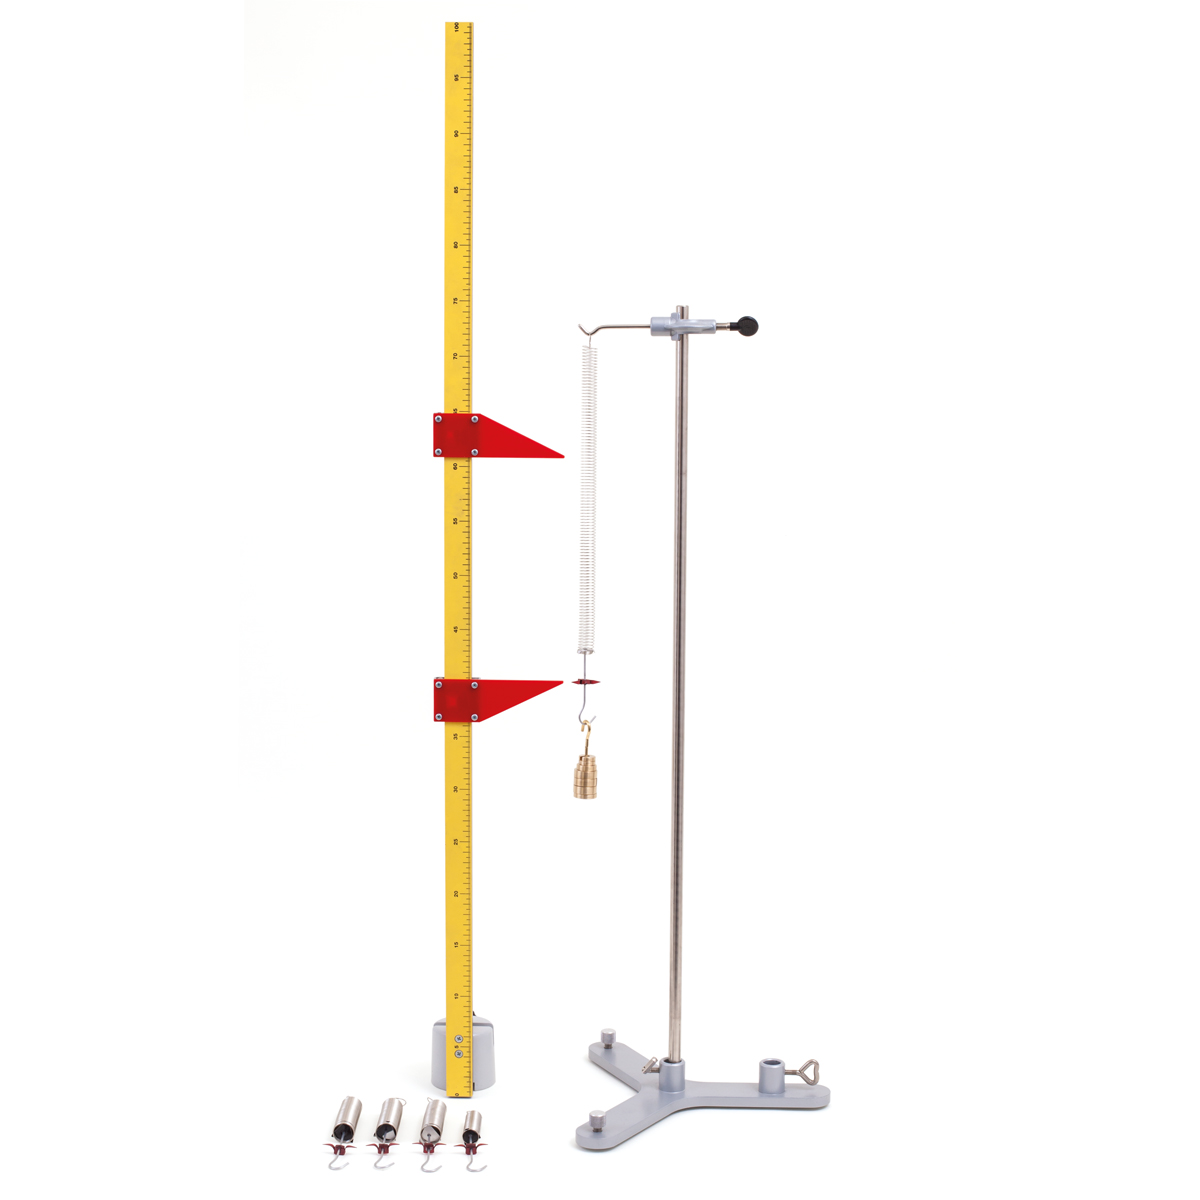
\includegraphics[width=0.95\linewidth]{Images/Ley de hooke.jpg}
    \caption{Montaje experimental para el método estático}
    \label{Montaje estatico}
\end{wrapfigure}

En primer lugar determinamos el valor de la constante elástica por el método estático, adoptando la configuración experimental que se puede ver en la Fig.\ref{Montaje estatico}.
Para determinar la constante decidimos tomar 10 medidas de la deformación que producen diez masas diferentes. Para ello realizaremos una regresión lineal simple sin término independiente por el método de los mínimos cuadrados, representando la fuerza en función de la deformación, ya que siguen una relación lineal como observamos en la Ec.\ref{Met estatico}. La pendiente de la recta ($F=\mathbf{b}\Delta x$) se corresponderá con la constante elástica del muelle. Las incertidumbres con las que trabajaremos en este caso son aquellas que proceden de nuestras medidas directas de las masas y las deformaciones.

\newpage

\begin{itemize}
    \item La incertidumbre de la masa viene dada por la precisión instrumental de la balanza y será la misma para todas las masas medidas de forma directa durante la práctica. Esta incertidumbre está directamente relacionada con la del peso:
    \begin{equation}
        s(m) = 0,01 \; g = 0,00001 \; kg \Rightarrow s(F) =9,8\cdot s(m) = 0,00098 \; N
        \label{Inc peso}
    \end{equation}
    \item La incertidumbre de la deformación viene dada por la precisión instrumental de la regla, que es de 1 mm. No obstante, en este caso consideramos que la incertidumbre es algo mayor, pues el aparato de medida y el muelle no estaban físicamente pegados y la incertidumbre dependerá de la precisión que tengamos a la hora de tomar las medidas. Es por ello que hemos decidido tomar como incertidumbre de la medida de la regla es de 2 mm. La deformación la mediremos de forma indirecta, fijando un valor de $x_0$ (El punto de equilibrio) como cero y medir lo que se deforma respecto de ese cero restando las medidas según la siguiente ecuación:
    \begin{equation}
        \Delta x = x - x_0
        \label{Deformación}
    \end{equation}

    Por tanto la incertidumbre de la deformación la obtenemos de forma indirecta a partir de la siguiente ecuación:

    \begin{equation}
        s(\Delta x) = \sqrt{\left (\frac{\partial \Delta x}{\partial x}\right )^2s^2(x) + \left (\frac{\partial \Delta x}{\partial x_0}\right )^2s^2(x_0)} = \sqrt{2s^2(x)} = 2\sqrt{2} = 2,8 \; mm
        \label{Inc deformacion}
    \end{equation}
\end{itemize}

El segundo método empleado para determinar la constante elástica fue el método dinámico, que se basa en la relación entre el período de oscilación y la masa que cuelga del muelle, como vimos en la Ec.\ref{Met dinamico}. Si elevamos ambos miembros de esta ecuación al cuadrado obtenemos la siguiente relación:

\begin{equation}
    T^2 = \frac{1}{k} 4 \pi^2 m
\end{equation}

De esta forma podemos ver que existe una clara relación lineal entre las magnitudes $T^2$ y $4\pi^2m$, donde $\frac{1}{k}$ es la pendiente de la propia recta. Para calcular la pendiente de esta recta realizaremos un ajuste simple sin término independiente ($y=bx$) por el método de los mínimos cuadrados de $T^2$ frente a  $4\pi^2m$. La incertidumbre asociada a la masa es la misma, por lo que la incertidumbre asociada a la variable independiente ($4\pi^2m$) es:

\begin{equation}
    s(4\pi^2m) = 4\pi^2s(m) = 0.39 \; g
\end{equation}

La medida del período de oscilación se realizó de forma directa con un cronómetro y para darle mayor fiabilidad a la medida cronometramos un intervalo de tiempo equivalente a diez períodos ($10T$). De esta forma reducimos en un orden de magnitud la incertidumbre de la medida al tener que dividirla entre 10. La incertidumbre de cada medida directa que tomamos ($10T$) será el tiempo de reacción medio de un ser humano, que manda frente a la precisión instrumental del cronómetro. El valor que tomaremos como referencia será el tiempo medio de reacción frente a un estímulo visual que es de $0,25$ s. Por tanto las incertidumbres correspondientes son:

\begin{equation}
    \begin{gathered}
        s(10T) = 0,25 \; s \Rightarrow s(T) = 0,025 \; s \\
        s(T^2) = \sqrt{\left (\frac{\partial T^2}{\partial T} \right )^2s^2(T)} = 2T\cdot s(T) = 0,05 \cdot T \; s
        \label{Inc T^2} 
    \end{gathered}
\end{equation}

A partir del ajuste podremos calcular el valor de la constante elástica del muelle y compararemos los resultados obtenidos por ambos métodos.

\subsection{Determinación de densidades de diferentes materiales}

En este apartado de la práctica trataremos de determinar la densidad de varios sólidos y un líquido. Para ello empleamos los siguientes materiales:


\begin{itemize}
    \item Muelle pendurado de un soporte
    \item Pesas de densidad desconocida y una balanza
    \item Un líquido de densidad conocida, agua, y otro de densidad desconocida, alcohol.
    \item Regla vertical para medir la deformación
\end{itemize}

Como explicamos en la introducción, nos vamos a valer del principio de Arquímedes para determinar diferentes densidades. El objetivo fundamental será cuantificar el efecto del empuje del líquido en la deformación, que será menor que en ausencia de líquido. Para ello mediremos la deformación que sufre el muelle cuando de él cuelga una masa $m$, $\Delta x$, y la deformación cuando esa misma masa $m$ está sumergida en un líquido de densidad conocida, $\Delta x'$. 

\newpage

\begin{wrapfigure}{l}{0.3\textwidth}
    \centering
    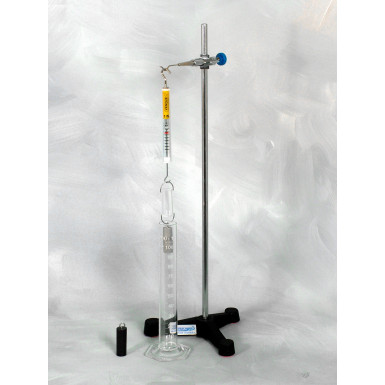
\includegraphics[width=0.95\linewidth]{Images/hooke+arquimedes.jpg}
    \caption{Montaje experimental para la determinación de densidades}
    \label{Hooke+arquimedes}
\end{wrapfigure}

El montaje experimental empleado puede verse en la siguiente figura. De esta forma podremos calcular la densidad del material del que está hecho esa misma masa $m$, aplicando la Ec.\ref{Densidad sol}. Para calcular la densidad de un líquido debemos realizar las mismas medidas con un sólido de densidad conocida (Usaremos la calculada anteriormente) y aplicaremos la Ec. \ref{Densidad liq}. La incertidumbre asociada a las deformaciones es la misma con la que trabajamos en el apartado anterior, reflejada en la Ec.\ref{Inc deformacion}. Por otro lado, tomaremos la densidad conocida como una constante y calcularemos la densidad del material desconocido a partir de propagación de incertidumbres:

\begin{itemize}
    \item Aplicando propagación de incertidumbres a la Ec.\ref{Densidad sol} obtenemos la incertidumbre de la densidad del sólido:
    \begin{equation}
        s(\rho_s)=\sqrt{\left (\frac{-\rho_L \Delta x'}{(\Delta x -\Delta x')^2} \right )^2s^2(\Delta x) + \left (\frac{\rho_L \Delta x}{(\Delta x - \Delta x')^2}\right )^2s^2(\Delta x')}
        \label{Inc densidad solido}
    \end{equation}
    \item Aplicando propagación de incertidumbres a la Ec.\ref{Densidad liq} obtenemos la incertidumbre de la densidad del líquido:
    \begin{equation}
        s(\rho_L) = \sqrt{ \left (\frac{\rho_s\Delta x'}{(\Delta x)^2}\right )^2s^2(\Delta x) + \left (\frac{-\rho_s}{\Delta x} \right )^2s^2(\Delta x') + \left (\frac{\Delta x -\Delta x'}{\Delta x}\right )^2s^2(\rho_s)}
        \label{Inc densidad liquido}
    \end{equation}
\end{itemize}

\subsection{Determinación del valor de la gravedad}

El último apartado de la práctica consiste en determinar el valor de la gravedad a partir de una caída libre controlada que suponemos ideal. El material empleado fue el siguiente:

\begin{itemize}
    \item Bola metálica
    \item Aparato dotado de un electroimán y un sensor de movimiento
    \item Regla milimetrada
\end{itemize}

\begin{wrapfigure}{r}{0.4\textwidth}
    \centering
    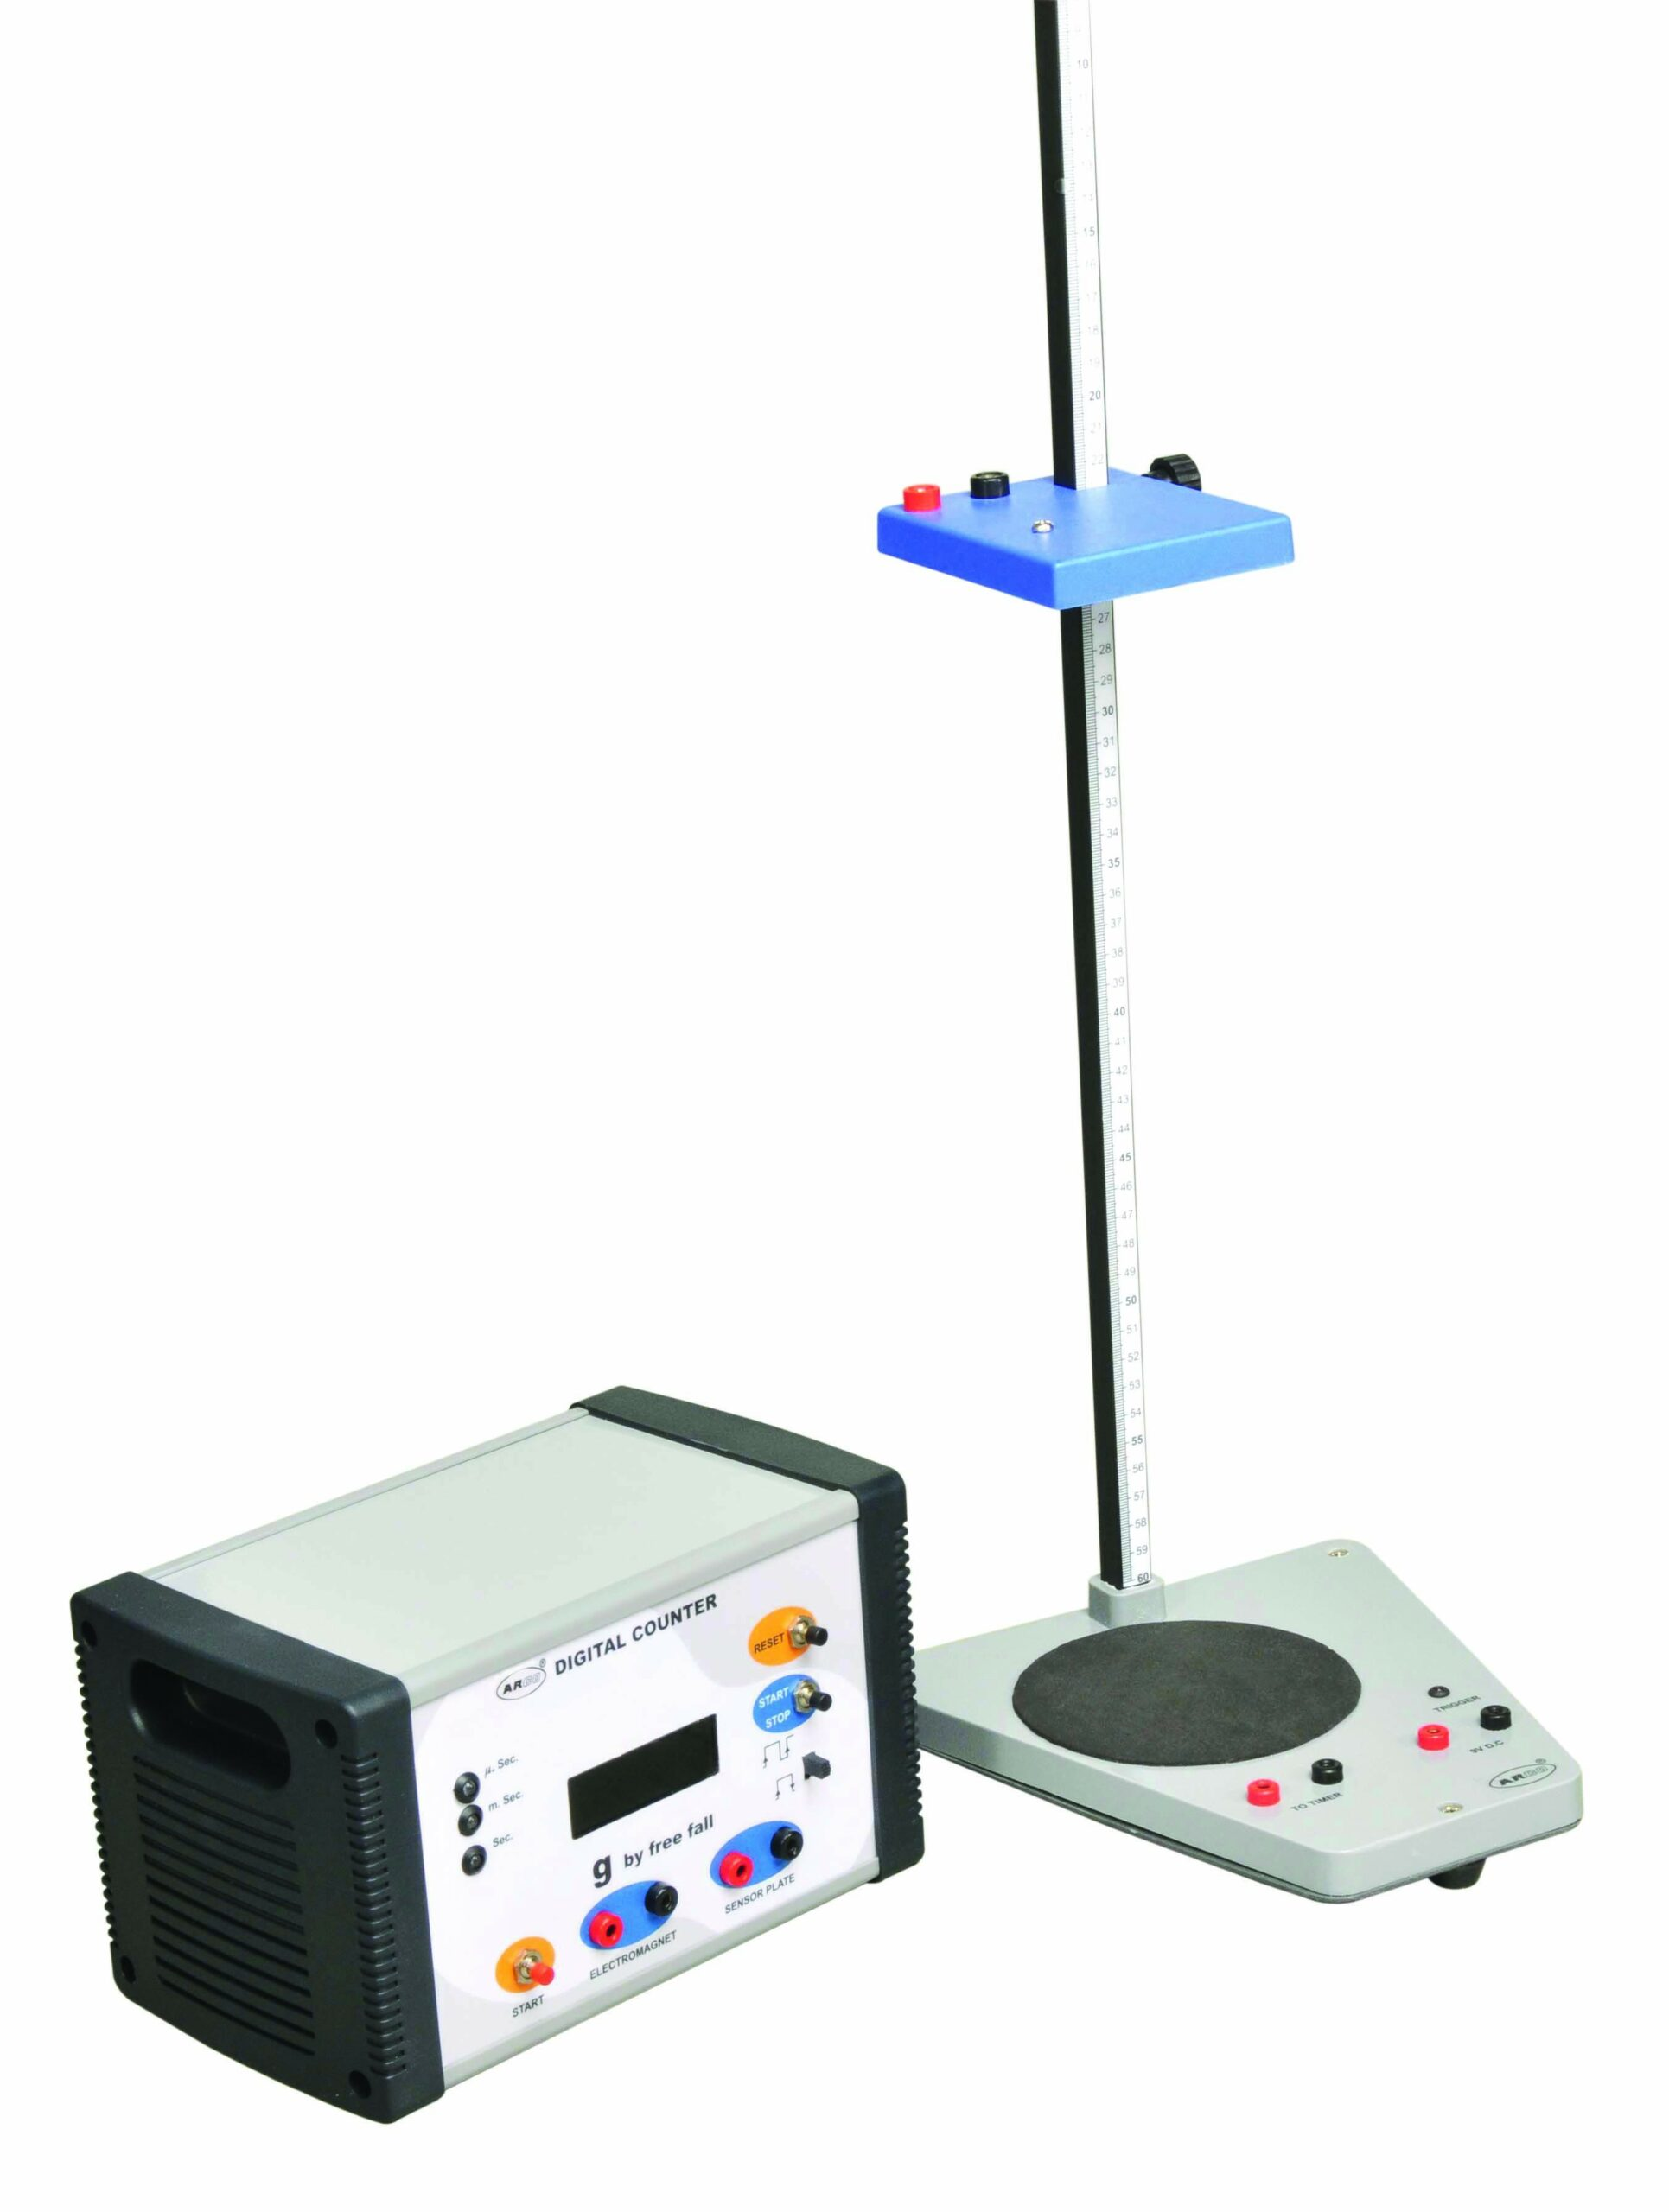
\includegraphics[width=0.7\linewidth]{Images/caidalibreaparato.jpg}
    \caption{Aparato para medir el tiempo de caída}
    \label{Montaje caida}
\end{wrapfigure}

El procedimiento llevado a cabo es muy sencillo, pues contábamos con un aparato de medida (Fig.\ref{Montaje caida}) dotado de un electroimán que soportaba la bola hasta que llegaba la señal para que se soltara y comenzaba nuestra caída libre. En ese preciso instante en que comenzaba la caída se activaba el contador del tiempo de caída gracias al sensor de movimiento, que paraba el contador cuando la bola llegaba a la base del aparato. Para calcular el valor de $g$ tomamos 10 medidas del tiempo de caída para diferentes alturas y realizamos una regresión lineal simple sin término independiente:

\begin{equation}
    t = \sqrt{\frac{2h}{g}} \Rightarrow 2h = gt^2
    \label{Ajuste gravedad}
\end{equation}

A partir de esta expresión ya tenemos nuestra relación lineal (Entre $2h$ y $t^2$) con la que podremos realizar nuestro ajuste por mínimos cuadrados a una recta del tipo $2h=bt^2$ donde la pendiente de la recta se corresponde con el valor de la gravedad. Las incertidumbres que debemos tener en cuenta son las siguientes:

\begin{itemize}
    \item La incertidumbre de la altura viene dada por la precisión instrumental de la regla:
    \begin{equation}
        s(h) = 0,001\; m \Rightarrow s(2h) = 0,002 \; m
    \end{equation}
    \item La incertidumbre del tiempo de caída viene dada por la incertidumbre del sensor, este valor nos ayudará a calcular la incertidumbre de $t^2$ a partir de propagación de incertidumbres:
    \begin{equation}
        s(t) = 0.00001 \; s \Rightarrow s(t^2)= 2t \cdot s(t) = 0.00002 \cdot t \; s
        \label{Inc Tcuadrado}
    \end{equation}
\end{itemize}

\newpage

\section{Análisis de datos}

\subsection{Determinación de la constante elástica del muelle}

\subsubsection{Método estático}

Como hemos mencionado anteriormente, para el método estático hemos tomado diez medidas de la deformación que producen diferentes masas. En la siguiente tabla podemos ver esos datos, así como la fuerza producida por esa masa:

\begin{table}[h!]
    \centering
    \begin{tabular}{|c|c|c|}
    \hline
    Masa (g) & F (N) ($F=mg$) & $\Delta x$ (m) \\ \hline
    10,20   & 0,09996 & 0,033 \\ \hline
    30,25  & 0,29645 & 0,099 \\ \hline
    50,27  & 0,49265 & 0,163 \\ \hline
    70,24  & 0,68835 & 0,227 \\ \hline
    80,20   & 0,78596 & 0,26  \\ \hline
    90,22  & 0,88416 & 0,291 \\ \hline
    100,01 & 0,98010 & 0,322 \\ \hline
    105,04 & 1,02939 & 0,340  \\ \hline
    110,07 & 1,07869 & 0,355 \\ \hline
    115,15 & 1,12847 & 0,372 \\ \hline
    \end{tabular}
    \caption{Datos experimentales medidos en el método estático}
    \label{Datos estatico}
\end{table}

A partir de la regresión lineal de $F$ frente a $\Delta x$ obtuvimos las siguientes magnitudes:

\begin{equation}
    \begin{gathered}
        b =  3.0335 \; N \cdot m^{-1} \\
        s(b) = 0.0026 \; N \cdot m^{-1} \\
        r =  0.999996 \\
        s =  0.0023
    \end{gathered}
\end{equation}

En la siguiente gráfica podemos ver respresentados los datos experimentales y la recta de regresión:

\newpage

\begin{figure}[h!]
    \centering
    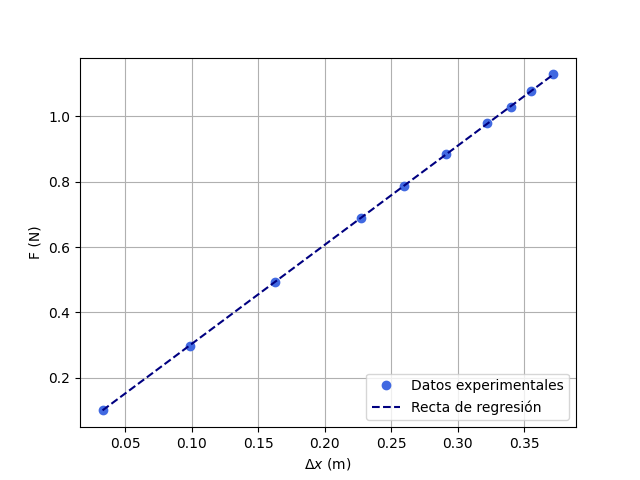
\includegraphics[width=0.75\linewidth]{Images/RegEstatico.png}
    \caption{Datos experimentales y recta de regresión del método estático}
\end{figure}

Finalmente, el valor de la constante elástica del muelle se corresponde con la pendiente de la recta, como demostramos antes, por lo que su valor es:

\begin{equation}
    k = 3.0335 \pm 0.0026 \; N \cdot m^{-1}
\end{equation}

\subsubsection{Método dinámico}

Para el método dinámico hemos tomado diez medidas del período de oscilación (En concreto de $10T$) para cada una de las masas empleadas anteriormente. Los datos recogidos figuran en la siguiente tabla acompañados de su respectiva incertidumbre, en el caso de $T^2$:

\newpage

\begin{table}[h!]
    \centering
    \begin{tabular}{|c|c|c|c|c|c|}
    \hline
    Masa (kg) & $4\pi^2m \; (kg)$ & $10T \; (s)$ & $T \; (s)$ & $T^2 \; (s^2) $&   $s(T^2) \; (s^2)$\\ \hline
    0,10200 & 4,02680  & 4,24  & 0,424 & 0,180 & 0,021 \\ \hline
    0,30250 & 11,94222 & 7,07  & 0,707 & 0,500 & 0,035 \\ \hline
    0,50270 & 19,84580 & 8,47  & 0,847 & 0,717 & 0,042 \\ \hline
    0,70240 & 27,72964 & 9,97  & 0,997 & 0,994 & 0,050 \\ \hline
    0,80200 & 31,66169 & 10,56 & 1,056 & 1,115 & 0,053 \\ \hline
    0,90220 & 35,61743 & 11,22 & 1,122 & 1,259 & 0,056 \\ \hline
    1,00010 & 39,48237 & 11,72 & 1,172 & 1,374 & 0,059 \\ \hline
    1,05040 & 41,46813 & 12,07 & 1,207 & 1,457 & 0,060 \\ \hline
    1,10070 & 43,45389 & 12,19 & 1,219 & 1,486 & 0,061 \\ \hline
    1,15150 & 45,45940 & 12,62 & 1,262 & 1,593 & 0,063 \\ \hline
    \end{tabular}
    \caption{Datos experimentales obtenidos a partir del método dinámico}
    \label{Datos dinamico}
    \end{table}

A partir de estos datos vamos a realizar nuestra regresión lineal de $T^2$ frente a $4\pi^2m$, como se ha mencionado anteriormente. Como los valores de $T^2$ presentan incertidumbres variables cabría la posibilidad de realizar un ajuste ponderado. No obstante, como la variación de las incertidumbres es pequeña, no llega siquiera a un orden de magnitud, vamos a realizar un ajuste simple, que nos proporcionará una aproximación muy buena del resultado. Los parámetros obtenidos fueron los siguientes:

\begin{equation}
    \begin{gathered}
        b = 0.3512 \; m\cdot N^{-1}\\
        s(b) = 0.0033 \; m\cdot N^{-1}\\
        r =  0.9996 \\
        s =  0.034
    \end{gathered}
\end{equation}

Como mencionamos anteriormente, la pendiente de esta recta es $\frac{1}{k}$, por lo que la constante elástica y su incertidumbre tienen la siguiente expresión:

\begin{equation}
    \begin{gathered}
        k = \frac{1}{b} = 2.847 \; N\cdot m^{-1} \\
        s(k) = \sqrt{\left (\frac{\partial k}{\partial b} \right )^2s^2(b)} = \frac{s(b)}{b^2} = 0.027 \; N\cdot m^{-1}
    \end{gathered}
\end{equation}

En la siguiente gráfica podemos ver una representación de los datos experimentales y de nuestra recta de regresión:

\begin{figure}[h!]
    \centering
    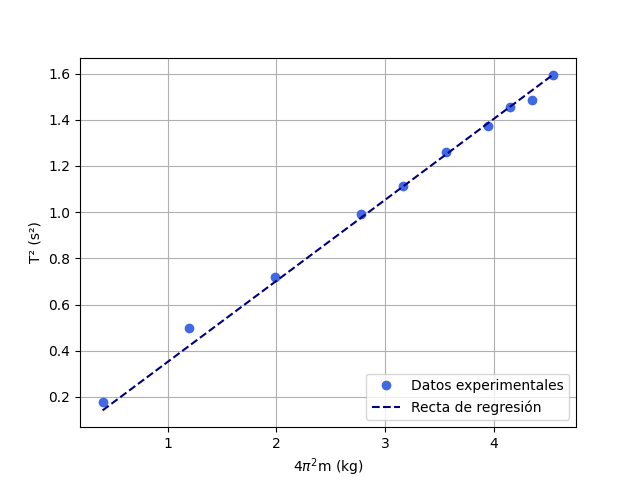
\includegraphics[width=0.75\linewidth]{Images/RegDinamico.png}
    \caption{Datos experimentales y recta de regresión del método dinámico}
\end{figure}

\newpage

Finalmente, podemos ver que el valor de nuestra constante difiere un poco al calculado por el método estático. Esta pequeña diferencia podría explicarse por el hecho de haber realizado una regresión lineal simple en vez de ponderada, que era lo que el problema pedía inicialmente al estar tratando con incertidumbres variables. Otra posible explicación de esta diferencia es un cierto error en la medida, pues muchas veces las oscilaciones no eran perfectas, si no que presentaban mucha irregularidad.



\subsection{Determinación de densidades}

\subsubsection{Sólidos}

Para la determinación de la densidad de sólidos contábamos con tres pesas de densidad desconocida, $m_1$, $m_2$ y $m_3$, y un líquido de densidad conocida, el agua $(\rho = 1000 \; kg\cdot m^{-3}=1 \; g\cdot mL^{-1})$. En la siguiente tabla podremos ver los valores de la deformación medidos ($\Delta x$), así como las deformaciones con los sólidos sumergidos en agua ($\Delta x'$), y la densidad y su incertidumbre (Calculadas a partir de la Ec.\ref{Densidad sol} y de la Ec.\ref{Inc densidad solido}):

\begin{table}[h!]
    \centering
    \begin{tabular}{c|c|c|c|c|}
    \cline{1-5}
    \multicolumn{1}{|c|}{Cuerpo}        & $\Delta x \; (m)$ & $\Delta x' \; (m)$ & $\rho_s \; (g\cdot cm^{-3})$ & $s(\rho_s) \; (g\cdot cm^{-3})$ \\ \hline
    \multicolumn{1}{|c|}{Plateado 1 ($46,26 \; g$)} & 0,160  & 0,102 & 8,40 & 0,59 \\ \hline
    \multicolumn{1}{|c|}{Plateado 2 ($137,87 \; g$)} & 0,445 & 0,392 & 2,76 & 0,16 \\ \hline
    \multicolumn{1}{|c|}{Dorado ($147,37 \; g$)} & 0,476 & 0,425 & 9,33 & 0,69 \\ \hline
    \end{tabular}
    \caption{Datos experimentales y cálculo de la densidad}
    \label{Datos dens sol}
\end{table}

\newpage

Para el contraste de resultados nos podemos fijar solo en un valor, el de la masa 2, que era la única hecha de un material conocido, aluminio. La densidad real del aluminio, según \textit{The Handbook of Chemistry and Physics}, es de $2,70 \; g\cdot cm^{-3}$, que está muy próximo al valor calculado experimentalmente y entra dentro de su rango de incertidumbre.

\subsubsection{Líquidos}

En este apartado tratamos de determinar la densidad, \textit{a priori} desconocida, de un líquido, el alcohol. Para ello tomamos las mismas medidas que en el apartado anterior, pero sumergiendo las tres mismas masas en alcohol en vez de en agua. De esta forma mediremos las diferentes deformaciones que se producen con las pesas al aire o sumergidas. Aplicando la Ec.\ref{Densidad liq} y la Ec.\ref{Inc densidad liquido} podemos calcular la densidad del alcohol con su incertidumbre asociada. Los valores obtenidos figuran en la siguiente tabla:

\begin{table}[h!]
    \centering
    \begin{tabular}{|c|c|c|c|c|}
    \hline
    Cuerpo &  $\Delta x \; (m)$ & $\Delta x' \; (m)$ & $\rho_{Al} \; (g\cdot m^{-3})$ & $s(\rho_{Al}) \; (g\cdot m^{-3})$\\ \hline
    Plateado 1 ($46,26 \; g$)& 0,160  & 0,130  & 0,517 & 0,062 \\ \hline
    Plateado 2 ($137,87 \; g$)& 0,445 & 0,398 & 0,887 & 0,062 \\ \hline
    Dorado ($147,37 \; g$) & 0,476 & 0,440  & 0,706 & 0,052 \\ \hline
    \end{tabular}
    \caption{Datos experimentales y cálculo de la densidad del alcohol}
    \label{Dens liquido}
    \end{table}

Según \textit{The Handbook of Chemistry and Physics} el valor real de la densidad del alcohol etílico, con el que trabajamos durante toda la práctica, es de $0,7893 \; gm \cdot cm^{-3}$. Si comparamos nuestros resultados con este valor podemos ver que las densidades obtenidas a partir de los datos de los dos últimos cuerpos se acercan bastante a este valor real, aunque presentan una cierta diferencia. Por otro lado, el valor de la densidad obtenido con el primer cuerpo se aleja enormemente de la realidad, por lo que posiblemente hayamos cometido algún error a la hora de tomar las medidas de la deformación de este cuerpo.

\subsection{Determinaación de la gravedad}

El último apartado de la práctica consistía en determinar el valor de la aceleración gravitatoria $g$ a partir de la caída libre ideal. Tomamos diez valores de referencia de tiempo de caída y altura, que representaremos en la siguiente tabla.Las incertidumbres de $t^2$ vienen dada spor la Ec.\ref{Inc Tcuadrado}:

\begin{table}[h!]
    \centering
    \begin{tabular}{|c|c|c|c|c|}
    \hline
    $h \; (m)$ & $2h \; (m)$ & $t \; (s)$ & $t^2 \; (s^2)$ & $s(t^2) \; (s^2)$ \\ \hline
    0,380 & 0,760 & 0,27488 & 0,0755590 & 0,0000055 \\ \hline
    0,400  & 0,800  & 0,28261 & 0,0798684 & 0,0000057 \\ \hline
    0,420 & 0,840 & 0,29176 & 0,0851239 & 0,0000058 \\ \hline
    0,460 & 0,920 & 0,29593 & 0,0875746 & 0,0000059 \\ \hline
    0,480 & 0,960 & 0,30416 & 0,0925133 & 0,0000061 \\ \hline
    0,500  & 1,000    & 0,31177 & 0,0972005 & 0,0000062 \\ \hline
    0,520 & 1,040 & 0,31880  & 0,1016334  & 0,0000064 \\ \hline
    0,540 & 1,080 & 0,32952 & 0,1085834  & 0,0000066 \\ \hline
    0,560 & 1,120 & 0,33338 & 0,1111422 & 0,0000067 \\ \hline
    0,580 & 1,160 & 0,34094 & 0,1162401 & 0,0000068 \\ \hline
    \end{tabular}
    \caption{Datos experimentales de la caída libre}
    \label{Datos gravedad}
\end{table}

A partir de estos datos vamos a realizar una regresión lineal por el método de los mínimos cuadrados de $2h$ frente a $t^2$ para conocer que el valor de $g$, que coincide con la pendiente de la recta. Como en la regresión realizada en el cálculo de $k$ por el método dinámico, cabría la posibilidad de realizar una regresión lineal ponderada. No obstante, la variación de las incertidumbres de $t^2$ es extremadamente pequeña, no llega siquiera al orden de magnitud, por lo que realizaremos una pequeña aproximación empleando una regresión simple sin término independiente. Las magnitudes obtenidas a partir del ajuste fueron las siguientes:

\begin{equation}
    \begin{gathered}
        b =  10.126 \; m \cdot s^{-2} \\
        s(b) = 0.063 \; m \cdot s^{-2} \\
        r =  0.9998 \\
        s =  0.019
    \end{gathered}
\end{equation}

En la siguiente figura podemos ver una representación gráfica de los datos experimentales, así como la recta de regresión:

\begin{figure}[h!]
    \centering
    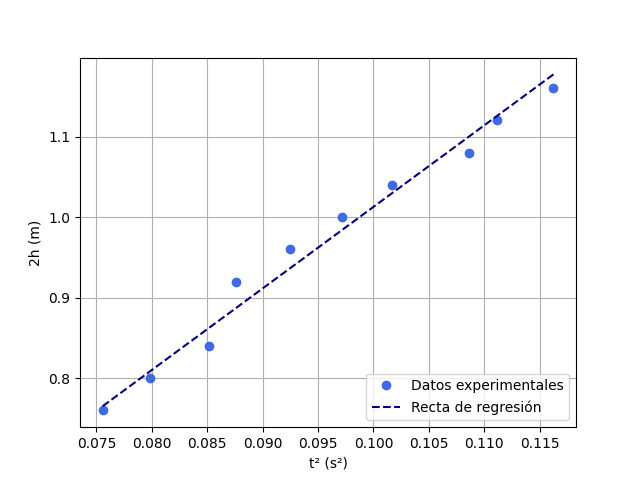
\includegraphics[width=0.75\linewidth]{Images/RegGravedad.png}
    \caption{Datos experimentales y regresión lineal de la caída libre}
\end{figure}

\newpage

Por tanto el valor final de la aceleración de la gravedad es:

\begin{equation}
    g = 10.126 \pm 0.063 \; m \cdot s^{-2}
\end{equation}

Este valor dista un poco del valor real de $9,807 \; m \cdot s^{-2}$, pero está dentro de un margen razonable para considerar al experimento como verídico.

\newpage

\section{Conclusiones}

Como conclusión, vamos a realizar una recopilación de todos los resultados obtenidos en los diferentes apartados de nuestra práctica, para poder realizar un análisis global de los resultados.

\par El primer apartado de la práctica se centró en calcular la constante elástica de nuestro muelle por el método dinámico y estático. Los resultados obtenidos fueron los siguientes:

\begin{table}[h!]
    \centering
    \begin{tabular}{|c|c|}
        \hline
        Método & $k \pm s(k) \; (N\cdot m^-1)$ \\ \hline
        Estático & $3,0335  \pm 0,0026$\\ \hline
        Dinámico & $2,847 \pm 0,027$\\ \hline
    \end{tabular}
\end{table}

Los resultados obtenidos parecen a simple vista más fiables en el método estático, por su incertidumbre menor, algo que podemos corrobar una vez realizado el experimento. En el método dinámico observamos que las oscilaciones estaban lejos de ser perfectas, presentabam mucha irregularidad, lo que dificultaba en parte tomar las medidas. Este hecho, ligado a que la incertidumbre debida al factor humano es mucho mayor empleando el método dinámico, nos hace sospechar en parte de este valor de la constante y tomar el valor obtenido en el método estático como referencia. Pese a todo los dos valores medidos no presentan siquiera diferencias superiores al $10\%$, por lo que podemos afirmar que nuestros resultados fueron satisfactorios.

\par En la segunda parte de la práctica tratamos de determinar las densidades de tres sólidos y un líquido a partir de la aplicación la ley de Hooke, comparando las deformaciones cuando sumergíamos los sólidos en un líquido y cuando los dejábamos al aire. 

\par Los resultados obtenidos para la densidad de los sólidos fueron:

\begin{table}[h!]
    \centering
    \begin{tabular}{|c|c|c|}
        \hline
        Cuerpo & $m \pm s(m) \; (g)$ & $\rho \pm s(\rho) \; (g\cdot m^{-3})$ \\ \hline
        Cuerpo 1 & $46,26 \pm 0,01$ & $8,40 \pm 0,59$ \\ \hline
        Cuerpo 2 & $137,87 \pm 0,01$ & $2,76 \pm 0,16$\\ \hline
        Cuerpo 3 & $147,37 \pm 0,01$& $9,33 \pm 0,69$ \\ \hline
    \end{tabular}
    \caption{Resultados de la densidad de los cuerpos con los que trabajamos}
\end{table}

Los resultados obtenidos para la densidad del alcohol con los diferentes sólidos fueron:

\begin{table}[h!]
    \centering
    \begin{tabular}{|c|c|c|}
        \hline
        Cuerpo & $m \pm s(m) \; (g)$ & $\rho_{Al} \pm s(\rho_{Al}) \; (g\cdot m^{-3})$ \\ \hline
        Cuerpo 1 & $46,26 \pm 0,01$ & $0,517 \pm 0,062$ \\ \hline
        Cuerpo 2 & $137,87 \pm 0,01$ & $0,887 \pm 0,062$\\ \hline
        Cuerpo 3 & $147,37 \pm 0,01$& $0,706 \pm 0,052$ \\ \hline
    \end{tabular}
    \caption{Resultados de la densidad del alcohol}
\end{table}

\newpage

Sobre los resultados obtenidos para los sólidos poco podemos decir sobre su precisión, pues salvo el caso ya comentado del cuerpo 2 (Hecho de aluminio), desconocíamos de que material estaban compuestos. No obstante, quizás podemos desconfiar del valor obtenido para el cuerpo 1, ya que el valor de la densidad del alcohol para ese cuerpo se aleja en gran medida de la realidad. Aunque esa desconfianza es solo una especulación, pues no podemos comprobar si el valor obtenido se ajusta a la realidad o no.

\par Por otro lado, los valores de la densidad del alcohol medidos, como ya comentamos tras el análisis de datos, cuentan con dos resultados aceptables y un resultado, el del cuerpo 1, que difiere enormemente de la realidad. El gran error en esa medida puede tener varias explicaciones, la primera y más obvia es un error humano a la hora de tomar las medidas. Otra posible causa de error es una falta de precisión arrastrada desde el apartado anterior. Para determinar la densidad del alcohol empleamos el valor de la densidad del cuerpo 1 calculado previamente.

\par En la última parte de la práctica tratamos de determinar el valor de la gravedad a partir del estudio de una caída libre ideal. El valor de la gravedad obtenido, comparado con el real, fue el siguiente:

\begin{table}[h!]
    \centering
    \begin{tabular}{c|c|}
    \cline{2-2}
                           & Valor de $g \; (m\cdot s^{-2})$\\ \hline
    \multicolumn{1}{|c|}{Experimental} &  $10,126 \pm 0,063$\\ \hline
    \multicolumn{1}{|c|}{Real} & $9,807$ \\ \hline
    \end{tabular}
    \caption{Resultado experimental de la aceleración de la gravedad}
    \label{tab:my-tabled}
    \end{table}

Como podemos observar, el valor de $g$ medido, pese a no estar dentro del intervalo de incertidumbre, se acerca bastante al valor teórico. Esta pequeña diferencia puede deberse a cierta falta de precisión a la hora de realizar el ajuste, ya que realizamos una regresión simple en lugar de ponderada, a pesar de que las incertidumbres de $t^2$ no cambiaban siquiera de orden de magnitud. Otra posible explicación para estas pequeñas diferencias es cierta falta de precisión a la hora de tomar las medidas, pues la precisión venía dada por el aparato de medida, que nosotros no controlábamos.

\newpage

\par En conclusión, pese a que en ciertas medidas obtuvimos un error considerable, podemos concluír que alcanzamos los objetivos principales de la práctica. Conseguimos determinar con éxito la constante elástica del muelle por el método estático y dinámico, conseguimos emplear ese mismo muelle para determinar la densidad de diferentes sólidos y un líquido y, por último, conseguimos determinar con éxito el valor de la gravedad a partir del estudio de una caída libre. Además de eso adquirimos una gran experiencia en la experimentación con cuerpos oscilatorios sometidos a una fuerza recuperada y en la aplicación de la ley de Hooke a diversas situaciones para las que \textit{a priori} no es útil.

\newpage

\section{Anexo: Análisis por mínimos cuadrados}

En este anexo detallaremos el procedimiento para realizar una regresión lineal simple sin término independiente por el método de los mínimos cuadrados, que aplicaremos durante todas las prácticas. En concreto detallaremos el análisis relizado para determinar la constante elástica del muelle por el método estático, en donde representamos la fuerza $F$ frente a la deformación $\Delta x$. La pendiente de nuestra recta ($F=b\Delta x$) se corresponde con la constante elástica del muelle. Las ecuaciones que empleamos para realizar el ajuste fueron las siguientes:

\begin{equation}
    b=\frac{\sum_{i}x_{i}y_{i}}{\sum_{i}x_{i}^2}
\end{equation}
\begin{equation}
    s=\sqrt{\frac{\sum_{i}(y_{i}-bx_{i})^2}{n-1}}
\end{equation}
\begin{equation}
    s(b)=\frac{s}{\sqrt{\sum_{i}x_{i}^2}}
\end{equation}
\begin{equation}
    r=\frac{\sum_{i}x_{i}y_{i}}{\sqrt{(\sum_{i}x_{i}^2)(\sum_{i}y_{i}^2)}}
\end{equation}

En la siguiente tabla detallaremos los datos empleados para realizar el análisis paso a paso:

\begin{table}[h!]
    \centering
    \begin{tabular}{cc|c|c|c|}
    \hline
    \multicolumn{1}{|c|}{$\mathbf{x_i}$} & $\mathbf{y_{i}}$ & $\mathbf{x_ {i}^2}$ & $\mathbf{y_{i}^2}$ & $\mathbf{x_{i}y_{i}}$ \\ \hline
    \multicolumn{1}{|c|}{10,2}   & 0,09996 & 104,04     & 0,00999 & 1,01959   \\ \hline
    \multicolumn{1}{|c|}{30,25}  & 0,29645 & 915,0625   & 0,08788 & 8,96761   \\ \hline
    \multicolumn{1}{|c|}{50,27}  & 0,49265 & 2527,0729  & 0,2427  & 24,76531  \\ \hline
    \multicolumn{1}{|c|}{70,24}  & 0,68835 & 4933,6576  & 0,47383 & 48,34984  \\ \hline
    \multicolumn{1}{|c|}{80,2}   & 0,78596 & 6432,04    & 0,61773 & 63,03399  \\ \hline
    \multicolumn{1}{|c|}{90,22}  & 0,88416 & 8139,6484  & 0,78173 & 79,76855  \\ \hline
    \multicolumn{1}{|c|}{100,01} & 0,9801  & 10002,0001 & 0,96059 & 98,0196   \\ \hline
    \multicolumn{1}{|c|}{105,04} & 1,02939 & 11033,4016 & 1,05965 & 108,12734 \\ \hline
    \multicolumn{1}{|c|}{110,07} & 1,07869 & 12115,4049 & 1,16356 & 118,73097 \\ \hline
    \multicolumn{1}{|c|}{115,15} & 1,12847 & 13259,5225 & 1,27344 & 129,94332 \\ \hline
                                 &         & $\sum x_i^2=69461,8505$ & $\sum y_i^2=6,67112$ & $\sum x_i y_i=680,72613$ \\ \cline{3-5} 
    \end{tabular}
    \caption{Datos empleados para realizar la regresión}
    \label{Datos regresion 1}
    \end{table}

A partir de estos valores ya podemos calcular la pendiente de nuestra recta de regresión, que se corresponderá con la constante elástica del muelle, y el coeficiente de regresión, que nos proporcionará una idea de la correlación de nuestras medidas. Cuanto más cerca esté de 1 el valor de $r$ la correlación entre nuestras medidas será mayor:

\begin{equation}
    \begin{gathered}
        b = 3,0335 \; N \cdot m^{-1} \\
        r = 0,999996
    \end{gathered}
\end{equation}

Como podemos observar, el valor de nuestro coeficiente de regresión está muy próximo de 1, por lo que podemos afirmar que existe una gran correlación entre los datos, presentando una clara relación lineal.

\par Una vez calculado el valor de la pendiente de la recta ($b$) ya podemos proceder a calcular las incertidumbres derivadas del ajuste, la desviación típica y la incertidumbre de la pendiente de la recta ($s(b)$). Para ello necesitamos conocer el valor de $\sum_i(y_i-bx_i)^2$, que calcularemos a partir de los datos de la siguiente tabla:

\begin{table}[h!]
    \centering
    \begin{tabular}{c|c|}
    \hline
    \multicolumn{1}{|c|}{$\mathbf{y_i-bx_i}$}  & $\mathbf{(y_i-bx_i)^2}$\\ \hline
    \multicolumn{1}{|c|}{-30,84174}   & 951,2129262 \\ \hline
    \multicolumn{1}{|c|}{-91,466925}  & 8366,198369 \\ \hline
    \multicolumn{1}{|c|}{-152,001399} & 23104,4253  \\ \hline
    \multicolumn{1}{|c|}{-212,384688} & 45107,2557  \\ \hline
    \multicolumn{1}{|c|}{-242,50074}  & 58806,6089  \\ \hline
    \multicolumn{1}{|c|}{-272,798214} & 74418,86556 \\ \hline
    \multicolumn{1}{|c|}{-302,400237} & 91445,90334 \\ \hline
    \multicolumn{1}{|c|}{-317,609448} & 100875,7615 \\ \hline
    \multicolumn{1}{|c|}{-332,818659} & 110768,2598 \\ \hline
    \multicolumn{1}{|c|}{-348,179055} & 121228,6543 \\ \hline
                                      & $\sum_i(y_i-bx_i)^2=$635073,1457 \\ \cline{2-2} 
    \end{tabular}
    \caption{Datos empleados para calcular $s$ y $s(b)$}
    \label{tab:my-table}
    \end{table}

\newpage
Una vez conocido este valor ya podemos calcular las incertidumbres que nos faltan, la desviación típica y la incertidumbre de la pendiente de la recta, que se corresponde con la incertidumbre de la constante elástica del muelle:

\begin{equation}
    \begin{gathered}
        s = 0,0023 \\
        s(b) = 0,0026 \; N\cdot m^{-1}
    \end{gathered}
\end{equation}

Para terminar el ajuste vamos a representar gráficamente los datos con los que trabajamos, en el eje X representaremos la deformación y en el eje Y representaremos los valores de la fuerza. Además de eso representaremos nuestra recta de regresión, de pendiente $b=3,0335\; N\cdot m^{-1}$

\begin{figure}[h!]
    \centering
    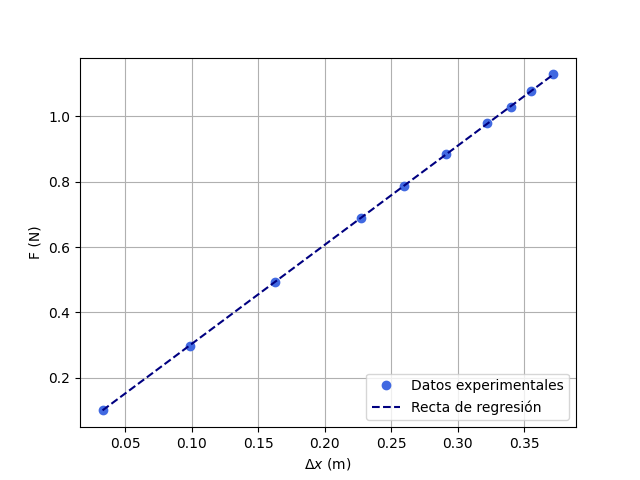
\includegraphics[width=0.75\linewidth]{Images/RegEstatico.png}
    \caption{Datos experimentales y recta de regresión obtenida a partir del ajuste}
\end{figure}

\chapter{Momento de inercia}

\section{Objetivos e introducción teórica}

Esta práctica gira alrededor del concepto de momento de inercia y tiene dos objetivos principales:

\begin{itemize}
    \item Medir experimentalmente el momento de inercia de diferentes cuerpos
    \item Verificar el teorema de Steiner
\end{itemize}

Para comenzar con nuestra práctica en primer necesitamos unas bases teóricas sobre las que realizar nuestros experimentos. La práctica parte del concepto de momento de inercia, magnitud que se define como la cuantificación de la inercia de rotación de un cuerpo. Matemáticamente el concepto de momento de inercia de un sistema de partículas se define como:

\begin{equation}
    I = \sum_i^N m_i r_i^2
\end{equation}

Esta fórmula puede generalizara para cuerpos de masa continua, que son con los que trabajamos, con la siguiente expresión:

\begin{equation}
    I = \int r^2 dm
    \label{Def MI}
\end{equation}

Si aplicamos esta expresión a determinados cuerpos geómetricos simples podemos obtener una expresión simplificada para su momento de inercia respecto a su eje de simetría:

\begin{equation}
    \begin{gathered}
        \text{Disco: } I=\frac{MR^2}{2} \\
        \text{Cilindro: } I = \frac{MR^2}{2}\\
        \text{Esfera: } I = \frac{2MR^2}{5} \\
        \text{Barra: } I = \frac{ML^2}{12}
        \label{MI cuerpos geometricos}
    \end{gathered}
\end{equation}

Siendo $M$ la masa del cuerpo, $R$ su radio y $L$ su longitud.
\par A partir de la definición de momento de inercia podemos intuir que esta magnitud va a presentar una gran relación con la rotación de los cuerpos y, por tanto, las magnitudes que la definen. Partiremos de la ecuación fundamental del movimiento de rotación:

\begin{equation}
    \vec{M} = \frac{d\vec{L}}{dt}
\end{equation}

Donde se relaciona el momento de la fuerza que produce la rotación ($\vec{M}=\vec{R}\times \vec{F}$) con la derivada del momento angular $\vec{L}$. En un sólido rígido el momento angular se puede expresar como:

\begin{equation}
    \vec{L} = I \vec{\omega}
\end{equation}

Siendo $\vec{\omega}$ la velocidad angular. Cuando el giro se produce sobre uno de los ejes principales del cuerpo el momento angular tiene la misma dirección que $\vec{\omega}$ y podemos emplear la expresión anterior en módulos ($L=I_e\omega$).

\par Para nuestra práctica mediremos el momento de inercia respecto a un eje a partir del período de oscilación de su rotación cuando se le hace girar sometido a la fuerza recuperadora de un resorte elástico. El momento de esa fuerza recuperadora cumple la siguiente relación:

\begin{equation}
    M = -D\varphi
    \label{Constante resorte}
\end{equation}

Donde $D$ es una constante propia del resorte y $\varphi$ es el ángulo girado. A partir de esta ecuación vamos a buscar una relación que nos permita calcular el momento de inercia del cuerpo respecto al eje a partir del momento de la fuerza, que podremos determinar experimentalmente:

\begin{equation}
    M = \frac{dL}{dt};\; L=I\omega;\; \omega = \frac{d\varphi}{dt} \Rightarrow M = I \frac{d^2\varphi}{dt^2}
\end{equation}

Teniendo en cuenta la expresión anterior y la Ec.\ref{Constante resorte} obtenemos la siguiente expresión:

\begin{equation}
    \frac{d^2\varphi}{dt^2} = -\frac{D}{I}\varphi
\end{equation}

Esta es la ecuación diferencial que describe el comportamiento de un oscilador simple, si la resolvemos obtenemos la siguiente expresión que nos ayuda a modelizar la oscilación:

\begin{equation}
    \varphi(t) = \varphi_0 \cos\left (\sqrt{\frac{D}{I}}t+\phi_0\right ) 
\end{equation}

El período de este movimiento armónico viene dado por la siguiente expresión:

\begin{equation}
    T = 2\pi\sqrt{\frac{I}{D}}
    \label{Periodo oscilacion}
\end{equation}

Esta expresión nos permitirá calcular el momento de inercia de nuestro cuerpo midiendo su período de oscilación cuando se somete a la fuerza recuperadora del resorte, algo mucho más fácil de medir experimentalmente. Esta igualdad nos servirá como fundamento para calcular todos los momentos de inercia medidos a lo largo de toda la práctica.

\par La segunda parte de la práctica se centra en verificar el teorema de Steiner, que afirma que el momento de inercia de un sólido rígido respecto a un eje es igual al momento de inercia respecto a otro eje paralelo que pasa por el centro de masas, más el producto de la masa del sólido por la distancia que separa ambos ejes al cuadrado. Matemáticamente se puede expresar como:

\begin{equation}
    I_{ee} = I_0 + md^2
    \label{Steiner}
\end{equation}

\section{Materiales y metodología}

Los materiales empleados para el estudio de sus propiedades fueron:

\begin{itemize}
    \item Disco perforado, de $381,39 \;g$ de masa y $29,9 \; cm$ de diámetro.
    \item Esfera maciza, de $659,23 \; g$ de masa y $13,8 \; cm$ de diámetro
    \item Cilindro macizo, de $384,29 \; cm $ de masa y $10 \; cm$ de diámetro
    \item Barra rígida, de $121.43 \;g$ de masa y $65,7 \; cm$ de longitud
\end{itemize}
La incertidumbre de las medidas masas viene dada por la precisión instrumental de la balanza:
\begin{equation}
    s(m) = 0,01 \; g
\end{equation}
Por otro lado, la incertidumbre de las medidas realizadas con la regla de los diámetros y la longitud de la barra viene dada por la precisión instrumental de la regla empleada:
\begin{equation}
    s(x) = 0,001 \;m
\end{equation}
Para realizar las medidas contamos con los siguientes instrumentos:

\begin{itemize}
    \item Balanza, con una precisión de 0,01 g
    \item Recta milimetrada, con una precisión de 0,001 m
    \item Soporte giratorio dotado de un resorte
    \item Detector fotoeléctrico empleado para medir semiperíodos
    \item Dinamómetro
\end{itemize}

En la siguiente figura podemos ver los materiales empleados:

\begin{figure}[h!]
    \centering
    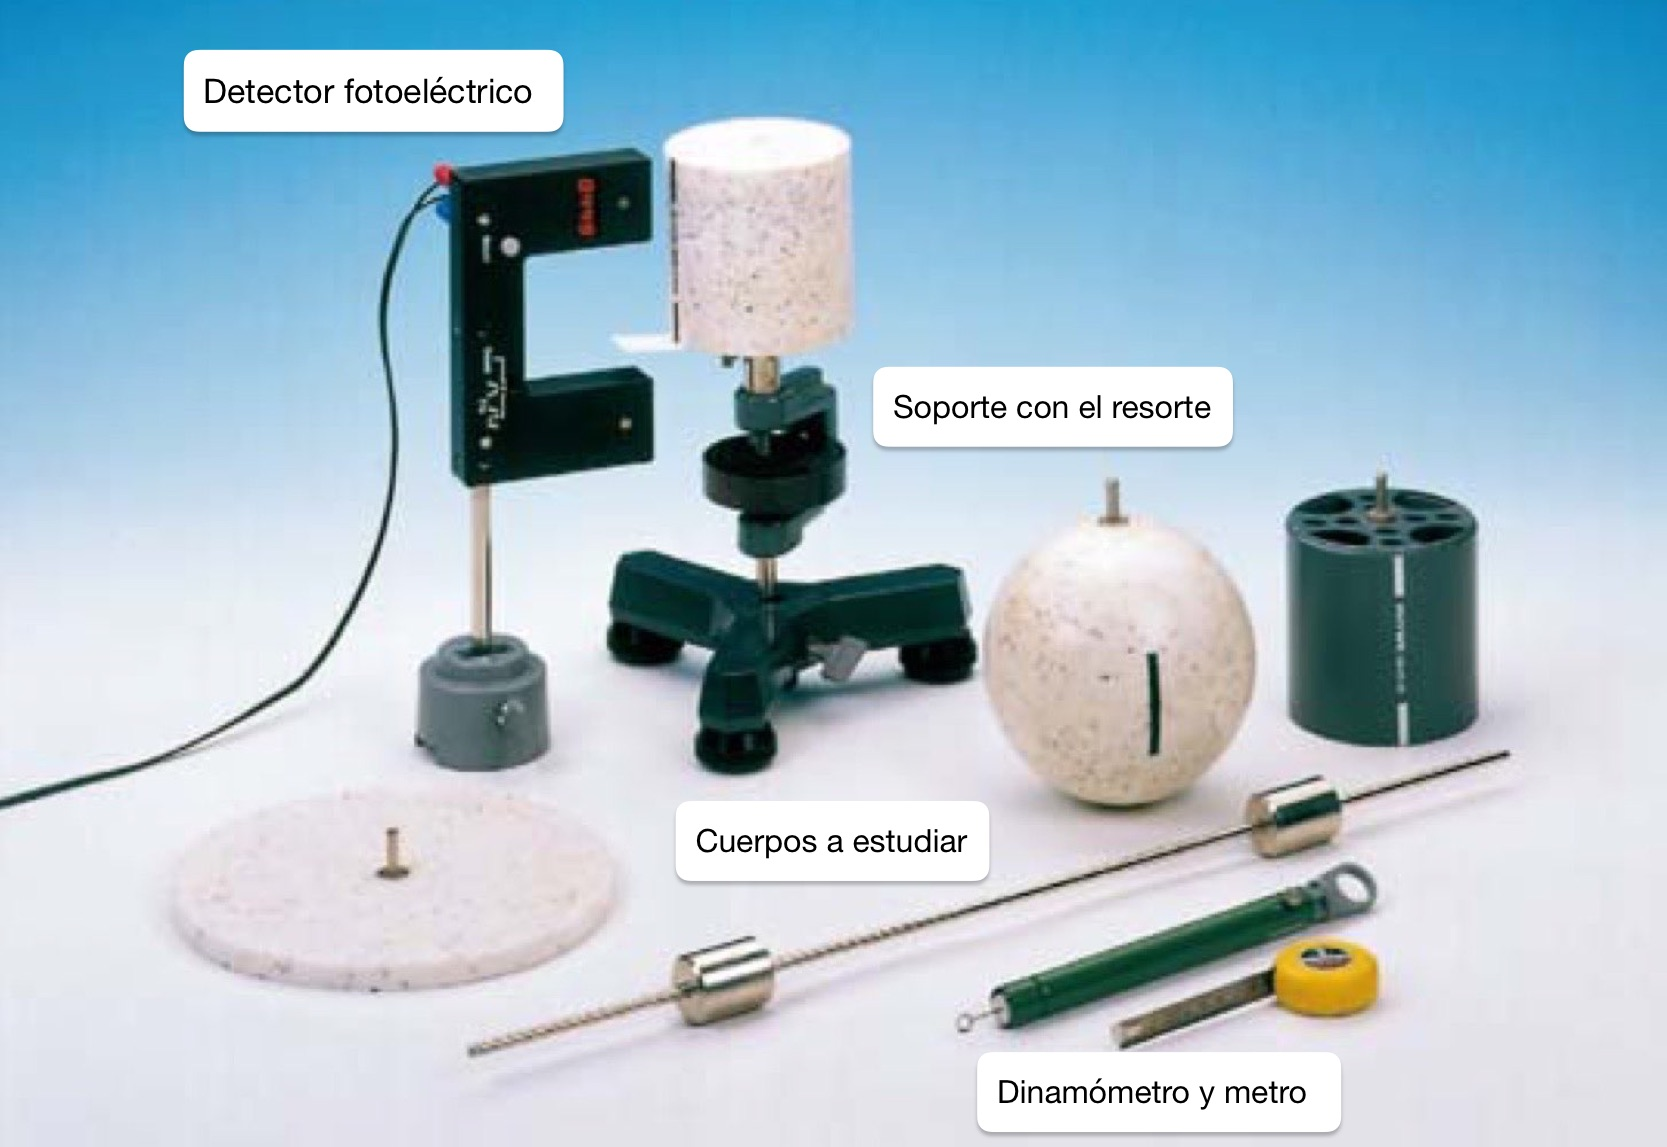
\includegraphics[width=0.75\linewidth]{Images/Material MI-1.jpg}
    \caption{Materiales empleados}
\end{figure}

\newpage

El procedimiento experimental seguido en cada una de las dos partes de la práctica se detallará a continuación:

\subsection{Determinación del momento de inercia de diferentes cuerpos}

Esta primera parte de la práctica se centra en determinar los momentos de inercia de diferentes cuerpos respecto a su eje de simetría. Para ello aplicaremos la Ec.\ref{Periodo oscilacion}, que relaciona el momento de inercia del cuerpo con su período de oscilación. No obstante, por comodidad a la hora de trabajar con el detector fotoeléctrico hemos decidido trabajar con semiperíodos. Por tanto la expresión de la Ec.\ref{Periodo oscilacion} se transforma en:

\begin{equation}
    T_{1/2} = \pi \sqrt{\frac{I}{D}}
    \label{SemiT osc}
\end{equation}

Como observamos en la expresión anterior la relación entre el semiperíodo y el momento de inercia depende también de la constante $D$ del resorte, \textit{a priori} desconocida. Para calcular el valor de esa constante partiremos de la Ec.\ref{Constante resorte} ($M=-D\varphi$R) y realizaremos un ajuste por mínimos cuadrados de $M$ frente s $\varphi$, donde la pendiente de la recta será la constante $D$. Para el ajuste tomaremos diez medidas con el dinámometro de la fuerza que es necesario ejercer para rotar el disco un determinado ángulo y, previo cálculo del momento de esas fuerzas, calcularemos la constante.

\par Para calcular los momentos de las fuerzas ejercidas vamos a suponer que el vector fuerza y el vector posición son perpendiculares, lo que nos permitirá trabajar solo con los módulos:

\begin{equation}
    M=RF
\end{equation}

Para la incertidumbre del momento aplicaremos propagación de incertidumbres:

\begin{equation}
    s(M) = \sqrt{F^2s^2(R)+R^2s^2(F)}
\end{equation}

Las incertidumbres involucradas son:

\begin{itemize}
    \item La incertidumbre de la fuerza aplicada, que viene dada por la precisión instrumental del dinamómetro:
    \begin{equation}
        s(F) = 0,01 \; N
    \end{equation}
    \item La incertidumbre del módulo del vector posición, que equivale al radio del disco. Este radio se obtuvo de forma indirecta, midiendo el diámetro del disco con la regla milimetrada que cuenta con una precisión instrumental de 1mm:
    \begin{equation}
        s(R) = \frac{s(d)}{2} = 0,0005 \; m
    \end{equation}
\end{itemize}

Las incertidumbre de los ángulos medidos viene dada por la precisión instrumental del disco:

\begin{equation}
    s(\varphi) = 5^\circ = 0,087 \;rad
\end{equation}

Una vez conocida la constantee $D$ del resorte podemos proceder a estudiar el semiperíodo de rotación bajo el efecto de la fuerza recuperadora del resorte. Para ello, como hemos mencioando anteriormente, mediremos varios valores del semiperíodo empleando el detector fotoeléctrico para poder tener una mejor estimación de su valor. Una vez tengamos nuestro valor de referencia del semiperíodo podremos aplicar la Ec.\ref{SemiT osc} para calcular el momento de inercia de cada cuerpo. En concreto la expresión empleada será:

\begin{equation}
    I = D \left (\frac{T_{1/2}}{\pi}\right )^2
    \label{Calculo MI figuras}
\end{equation}

A partir de propagación de incertidumbres podemos calcular la incertidumbre del momento de inercia experimental:

\begin{equation}
    \begin{gathered}
        s(I) = \sqrt{\left (\frac{\partial I}{\partial D}\right )^2s^2(D) + \left (\frac{\partial I}{\partial T_{1/2}}\right )^2s^2(T_{1/2})}\\
        s(I) = \sqrt{\left (\frac{T_{1/2}}{\pi}\right )^4s^2(D) + \left (\frac{2T_{1/2}D}{\pi^2}\right )^2s^2(T_{1/2})}
        \label{Inc MI figuras}
    \end{gathered}
\end{equation}

Las incertidumbres que participan en esta expresión son:

\begin{itemize}
    \item La incertidumbre de la constante $D$ del resorte, que la obtendremos a partir del ajuste por mínimos cuadrados mencionado anteriormente.
    \item La incertidumbre del semiperíodo de rotación, que viene dada por la precisión instrumental del detector fotoeléctrico:
    \begin{equation}
        s(T_{1/2}) = 0,001 \;s
    \end{equation}
\end{itemize}

\newpage

Una vez calculados los momentos de inercia experimentales de cada cuerpo debemos compararlos con el valor teórico, calculado a partir de la Ec.\ref{MI cuerpos geometricos} para cada figura concreta. Estos valores teóricos también cuentan con una incertidumbre asociada, pues se calculan en función de las dimensiones de la figura, medidas con la regla milimetrada, y de la masa, medida con la balanza. A continuación detallaremos cuál será la incertidumbre del momento de inercia de cada figura con la que trabajamos, calculadas a partir de propagación de incertidumbres:

\begin{itemize}
    \item El momento de inercia del disco es $\frac{MR^2}{2}$, siendo $M$ su masa y $R$ su radio, por lo que el valor teórico con su incertidumbre es:
    \begin{equation}
        \begin{gathered}
            I_D = 0.004262 \; kg \cdot m^2\\
            s(I_D) = \sqrt{\left (\frac{\partial I_D}{\partial M}\right )^2s^2(M) + \left (\frac{\partial I_D}{\partial R}\right )^2s^2(R)} \\ s(I_D)= \sqrt{\left (\frac{R^2}{2}\right )^2s^2(M) + (MR)^2s^2(R)} = 0.000074 \;kg\cdot m^2
        \end{gathered}
    \end{equation}
    \item El momento de inercia del cilindro tiene la misma ecuación ($\frac{MR^2}{2}$), por lo que aplicando la ecuación anterior con las dimensiones del cilindro obtenemos su momento de inercia con la incertidumbre asociada:
    \begin{equation}
        \begin{gathered}
            I_C = 0.00048036 \; kg \cdot m^2\\
            s(I_C) = 0.00000025 \; kg \cdot m^2
        \end{gathered}
    \end{equation}
    \item El último cuerpo con el que trabajamos en esta parte de la práctica fue la esfera, cuyo momento de inercia es $\frac{2MR^2}{5}$, por lo que el valor teórico con su incertidumbre asociada es de:
    \begin{equation}
        \begin{gathered}
            I_E = 0.000726 \; kg \cdot m^2 \\
            s(I_E) = \sqrt{\left (\frac{2R^2}{5}\right )^2s^2(M) + \left (\frac{4MR}{5}\right )^2s^2(R)} = 0,000045 \; kg\cdot m^2
        \end{gathered}
    \end{equation}
\end{itemize}

\newpage

\subsection{Verificación del teorema de Steiner}

En esta segunda parte de la práctica trataremos de verificar el teorema de Steiner (Ec.\ref{Steiner}). Para ello estudiaremos el momento de inercia respecto a varios ejes de dos cuerpos, el disco perforado y la varilla metálico. El disco perforado era el del apartado anterior, por lo que sus dimensiones son las mismas. La barra metálica tiene un longitud de $65,7$ cm de longitud y una masa de $0,12143 \; kg$.

\par Para verficar la igualdad del teorema vamos a realizar una regresión lineal de $I$ frente a $d^2$, la pendiente de esa recta será la masa $m$ del cuerpo y el término independiente será $I_0$. Para ello mediremos diez valores del semiperíodo (Para calcular $I$) con los cuerpos rotando alrededor de varios ejes. En primer lugar mediremos 10 semiperíodos con el cuerpo rotando sobre el eje por el que pasa por el centro de masas para calcular $I_0$. Luego realizaremos este mismo procedimiento con el cuerpo rotando sobre ejes situados a una distancia $d$ del eje paralelo que pasa por el centro de masas.

\par En el caso del disco perforado tomaremos 4 conjuntos de medidas, fijando el disco sobre cada una de las perforaciones, que se sitúan a distancias de 3, 6, 9 y 12 cm del centro de masas respectivamente, como se puede ver en la siguiente figura.

\begin{figure}[h!]
    \centering
    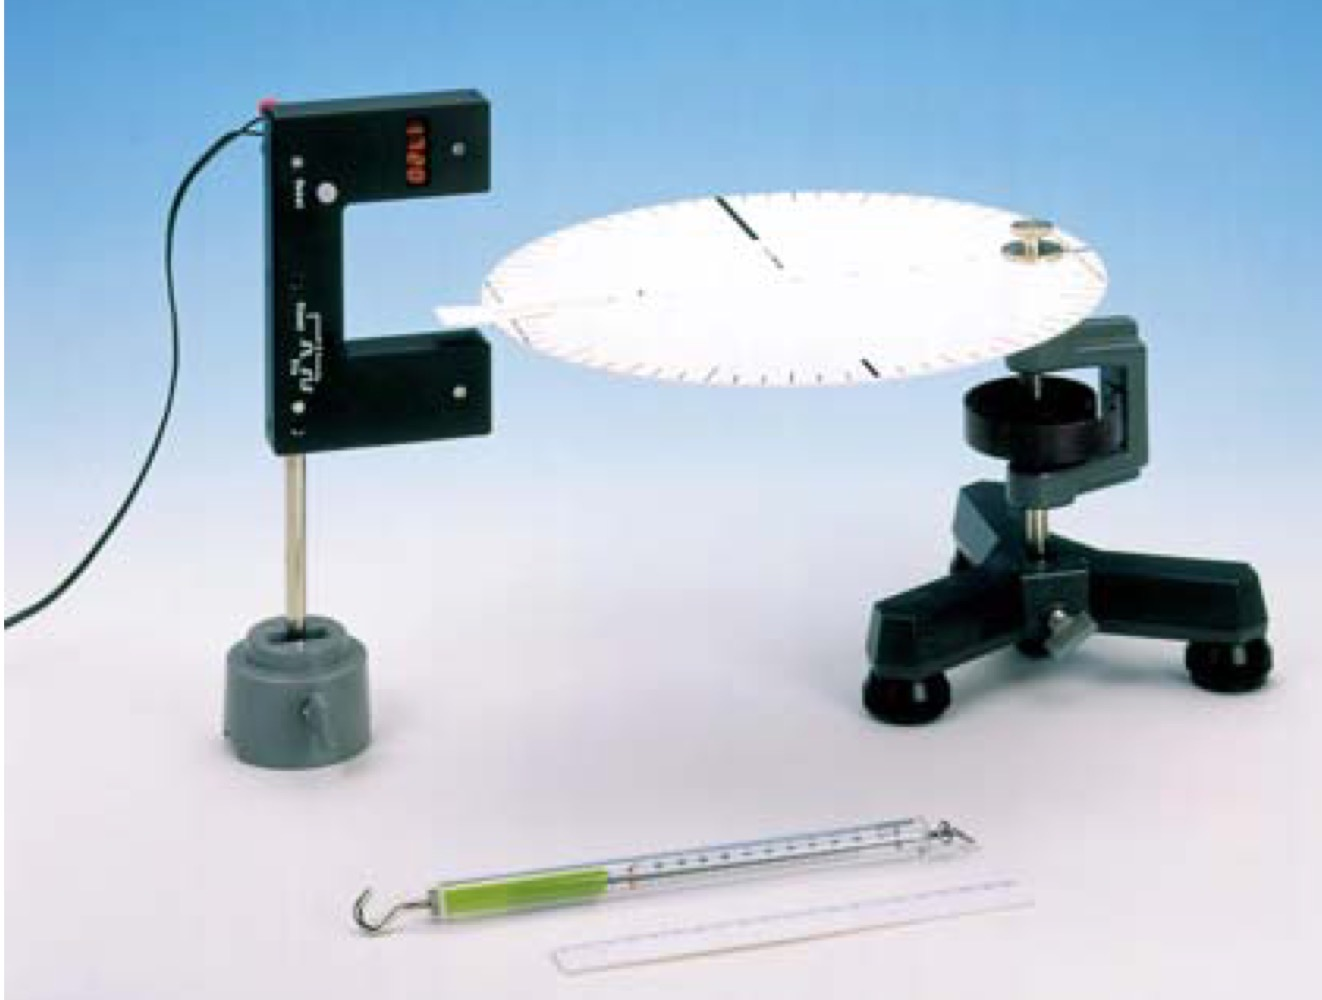
\includegraphics[width=0.65\linewidth]{Images/Material MI 2.jpeg}
    \caption{Montaje experimental para verificar el teorema de Steiner con el disco}
\end{figure}



\par En el caso de la varilla tomaremos 10 conjuntos de medidas, fijando la varilla sobre cada una de las perforaciones transversales con las que cuenta la varilla, situadas a 1 cm la una de la otra. Por tanto las distancias irán de 1 a 10 cm, aumentando de uno en uno. Cabe destacar que en esta parte de la práctica solo pudimos tomar 5 medidas del semiperíodo para cada valor de distancia por problemas técnicos. El problema observado fue que los valores medidos de los semiperíodos no resultaban nada fiables, oscilaban con frecuencia y en muchos momentos perdían la linealidad, por lo que es posible que los resultados en esta parte de la práctica no sean los esperados.


\section{Análisis de datos}

\subsection{Determinación del momento de inercia de diferentes cuerpos}

En la siguiente tabla podemos ver representadas las medidas tomadas en el laboratorio de los ángulo de rotación del disco y las fuerzas, con sus momentos asociados (Teniendo en cuenta que el radio del disco es $14,95 \; cm$), necesarias para producir esas rotaciones:

\begin{table}[h!]
    \centering
    \begin{tabular}{|c|c|c|c|c|c|}
    \hline
    Medida & $F \; (N)$ & $\varphi \; (^{\circ})$ & $\varphi \; (rad)$ & $M \; (N\cdot m)$ & $s(M) \; (N\cdot m)$ \\ \hline
    1  & 0,19 & 90  & 1,571 & 0,0284 & 0,0015 \\ \hline
    2  & 0,23 & 100 & 1,745 & 0,0344 & 0,0015 \\ \hline
    3  & 0,24 & 105 & 1,833 & 0,0359 & 0,0015 \\ \hline
    4  & 0,25 & 115 & 2,007 & 0,0374 & 0,0015 \\ \hline
    5  & 0,27 & 120 & 2,094 & 0,0404 & 0,0015 \\ \hline
    6  & 0,29 & 130 & 2,269 & 0,0434 & 0,0015 \\ \hline
    7  & 0,31 & 145 & 2,531 & 0,0463 & 0,0015 \\ \hline
    8  & 0,33 & 160 & 2,793 & 0,0493 & 0,0015 \\ \hline
    9  & 0,34 & 165 & 2,880 & 0,0508 & 0,0015 \\ \hline
    10 & 0,4  & 180 & 3,142 & 0,0598 & 0,0015 \\ \hline
    \end{tabular}
    \caption{Datos empleados para calcular la constante del resorte}
    \label{Tabla D resorte}
\end{table}

A partir de estos datos vamos a realizar una regresión lineal simple por el método de los mínimos cuadrados para ajustar $M$ frente a $\varphi$, donde la pendiente de esa recta será la constante $D$ del muelle. Cabe destacar que en la Ec.\ref{Constante resorte} aparece el signo menos porque $M$ actúa como el momento de una fuerza recuperadora, pero nosotros ajustaremos nuestros valores a la recta $M=D\varphi$. Los datos obtenidos a partir del ajuste son:

\begin{equation}
    \begin{gathered}
        b = 0.01857 \; N\cdot m \cdot rad^{-1}\\
        s(b) =  0.00024 \; N\cdot m \cdot rad^{-1}\\
        r =  0.9992 \\
        s =  0.0017
    \end{gathered}
\end{equation}

Por tanto el valor de la constante $D$ del resorte es:

\begin{equation}
    D = 0.01857 \pm 0.00024 \; N\cdot m \cdot rad^{-1}
\end{equation}

Una vez realizado este cálculo podemos empezar a determinar los diversos momentos de inercia.

\subsection{Determinación de los momentos de inercia de diferentes cuerpos}

Para determinar el momento de inercia de diferentes los diferentes cuerpos a estudiar aplicaremos la Ec.\ref{Calculo MI figuras}. Para ello necesitaremos conocer el semiperíodo de oscilación de los diferentes cuerpos, que estimaremos a partir de un conjunto de 15 medidas, para tener más fiabilidad.

\subsubsection{Disco}

En la siguiente tabla podemos ver las 15 medidas del semiperíodo del disco:

\begin{table}[h!]
    \centering
    \begin{tabular}{|c|c|c|c|c|c|}
    \hline
    Medida  &  $T_{1/2} \; (s)$ & Medida   &   $T_{1/2} \; (s)$    & Medida   &   $T_{1/2} \; (s)$    \\ \hline
    1 & 1,429 & 6  & 1,445 & 11 & 1,417 \\ \hline
    2 & 1,441 & 7  & 1,441 & 12 & 1,415 \\ \hline
    3 & 1,446 & 8  & 1,431 & 13 & 1,406 \\ \hline
    4 & 1,449 & 9  & 1,425 & 14 & 1,406 \\ \hline
    5 & 1,446 & 10 & 1,424 & 15 & 1,428 \\ \hline
    \end{tabular}
    \caption{Datos de los semiperíodos del disco}
    \label{SemiT disco}
\end{table}

Para determinar un valor de referencia para el semiperíodo vamos a realizar un tratamiento estadístico a los datos que nos permitirá escoger un valor fiable. En primer lugar calcularemos la media y la desviación típica de la muestra:

\begin{equation}
    \begin{gathered}
        \overline{T}_{1/2} = 1.4299 \; s\\
        s_A(T_{1/2}) = 0.014 \; s
    \end{gathered}
\end{equation}

A partir de estos datos estableceremos un intervalo de confianza centrado en el valor medio para evaluar los posibles valores discordantes a eliminar. Este intervalo vendrá dado por la siguiente expresión: $\overline{T}_{1/2} \pm k\cdot s_A(T_{1/2})$.Donde $k$ es el factor de cobertura, que con $k=2$ nos dará una confianza del $95\%$. En nuestro caso el intervalo será:

\begin{equation}
    1,4019 \; s \leq x_i \leq 1,4579 \; s
\end{equation}

Como podemos ver, todos los datos entran en nuestro intervalo por lo que no necesitamos eliminar ninguno. El siguiente paso será calcular la desviación típica de la media, así como la incertidumbre combinada:

\begin{equation}
    \begin{gathered}
        s_A(\overline{T}_{1/2}) = 0.0036 \; s\\
        s_C(\overline{T}_{1/2}) = 0.0037 \; s
    \end{gathered}
\end{equation}

Por tanto nuestro valor final de referencia del semiperíodo y su incertidumbre es:

\begin{equation}
    T_{1/2} = 1.4299 \pm 0.0037 \; s
\end{equation}

Si aplicamos la Ec.\ref{Calculo MI figuras} para calcular el valor del momento de inercia y la Ec.\ref{Inc MI figuras} para calcular su incertidumbre obtenemos:

\begin{equation}
    I_D = 0.003847 \pm 4.9 \cdot 10^{-5} \; kg\cdot m^2
\end{equation}

Comparando este valor con el teórico, de $0,004262 \; kg \cdot m^2$ podemos ver que, aunque no entra en el rango de incertidumbre, el resultado se acerca bastante a los esperado.

\subsubsection{Cilindro}

En la siguiente tabla podemos ver las medidas tomadas en el laboratorio del semiperíodo del cilindro:

\begin{table}[h!]
    \centering
    \begin{tabular}{|c|c|c|c|c|c|}
    \hline
    Medida  &  $T_{1/2} \; (s)$ & Medida   &   $T_{1/2} \; (s)$    & Medida   &   $T_{1/2} \; (s)$    \\ \hline
    1 & 0,436 & 6  & 0,436 & 11 & 0,433 \\ \hline
    2 & 0,435 & 7  & 0,438 & 12 & 0,437 \\ \hline
    3 & 0,431 & 8  & 0,435 & 13 & 0,435 \\ \hline
    4 & 0,429 & 9  & 0,435 & 14 & 0,435 \\ \hline
    5 & 0,432 & 10 & 0,433 & 15 & 0,435 \\ \hline
    \end{tabular}
    \caption{Datos del semiperíodo del cilindro}
    \label{Datos semiT cilindro}
\end{table}

Para determinar un valor de referencia del semiperíodo del cilindro vamos a realizar el mismo tratamiento estadístico que realizamos en el apartado anterior. La media y la desviación típica de la muestra son:

\begin{equation}
    \begin{gathered}
        \overline{T}_{1/2} = 0.4344 \; s\\
        s_A(T_{1/2}) = 0.0022 \; s
    \end{gathered}
\end{equation}

Si establecemos nuestro intervalo de confianza aplicando el factor de cobertura $k=2$, que en este caso será el intervalo $(0,4300 \leq x_i \leq 0.4388)$, podemos ver que el dato $T_{1/2}=0,429 \; s$ se queda fuera, por lo que lo descartaremos. Una vez descartado este valor vamos a calcular la nueva media y la desviación típica final de la media, así como la incertidumbre combinada:

\begin{equation}
    \begin{gathered}
        \overline{T}_{1/2} = 0.43480 \; s \\
        s_A(\overline{T}_{1/2}) = 0.00046 \; s \\
        s_C(\overline{T}_{1/2}) = 0.0011 \; s
    \end{gathered}
\end{equation}

Por tanto, nuestro valor de referencia del semiperíodo con su incertidumbre es:

\begin{equation}
    T_{1/2} = 0.4348 \pm 0.0011 \; s
\end{equation}

Si aplicamos la Ec.\ref{Calculo MI figuras} para calcular el valor del momento de inercia y la Ec.\ref{Inc MI figuras} para calcular su incertidumbre obtenemos:

\begin{equation}
    I_C = 0.0003557 \pm 4.8 \cdot 10^{-6} \; kg\cdot m^2
\end{equation}

Comparando este resultado con el valor teórico de $0,00048036 \; kg \cdot m^2$ podemos ver que presentan una pequeña diferencia, no entra dentro del rango de incertidumbre que determinamos a partir de nuestro análisis estadístico.

\newpage

\subsubsection{Esfera}

En la siguiente tabla podemos ver las medidas tomadas en el laboratorio del semiperíodo del cilindro:

\begin{table}[h!]
    \centering
    \begin{tabular}{|c|c|c|c|cc}
    \hline
    Medida  &  $T_{1/2}\; (s)$ & Medida   & $T_{1/2}\; (s)$   & \multicolumn{1}{c|}{Medida}   & \multicolumn{1}{c|}{$T_{1/2}\; (s)$}      \\ \hline
    1 & 0,727 & 6  & 0,728 & \multicolumn{1}{c|}{11} & \multicolumn{1}{c|}{0,729} \\ \hline
    2 & 0,726 & 7  & 0,727 & \multicolumn{1}{c|}{12} & \multicolumn{1}{c|}{0,729} \\ \hline
    3 & 0,727 & 8  & 0,729 & \multicolumn{1}{c|}{13} & \multicolumn{1}{c|}{0,728} \\ \hline
    4 & 0,727 & 9  & 0,729 &                         &                            \\ \cline{1-4}
    5 & 0,726 & 10 & 0,73  &                         &                            \\ \cline{1-4}
    \end{tabular}
    \caption{Datos del semiperíodo de la esfera}
    \label{Datos semiT esfera}
\end{table}



Para determinar un valor de referencia del semiperíodo del cilindro vamos a realizar el mismo tratamiento estadístico que realizamos en el apartado anterior. La media y la desviación típica de la muestra son:

\begin{equation}
    \begin{gathered}
        \overline{T}_{1/2} = 0.7278 \; s\\
        s_A(T_{1/2}) = 0.0012 \; s
    \end{gathered}
\end{equation}

Si establecemos nuestro intervalo de confianza aplicando el factor de cobertura $k=2$, que en este caso será el intervalo $(0,7254 \leq x_i \leq 0.7302)$, podemos ver que todos los datos están dentro del intervalo, por lo que no tenemos que descartar ninguno. La desviación típica de la media y la incertidumbre combinada tienen los siguientes valores:

\begin{equation}
    \begin{gathered}
        s_A(\overline{T}_{1/2}) = 0.00034 \; s\\
        s_C(\overline{T}_{1/2}) = 0.0010 \; s
    \end{gathered}
\end{equation}

Después de este tratamiento de los datos ya tenemos nuestro valor de referencia del semiperíodo de la esfera con su incertidumbre:

\begin{equation}
    T_{1/2} = 0.7278 \pm 0.0010 \; s
\end{equation}

Si aplicamos la Ec.\ref{Calculo MI figuras} para calcular el valor del momento de inercia y la Ec.\ref{Inc MI figuras} para calcular su incertidumbre obtenemos:

\begin{equation}
    I_E = 0.000997 \pm  1,3 \cdot 10^{-5} \;kg\cdot m^2
\end{equation}

Comparando este valor con el valor teórico, de $0,000726 \; kg \cdot m^2$, podemos ver una pequeña diferencia. Estas pequeñas diferencias entre el valor teórico del momento de inercia y el medido experimentalmente se repiten de forma reiterada durante toda la práctica, como podemos ver comparando resultados. Este fenómeno puede tener diversas causas, pero la que creemos más probable es la falta de homogeneidad en los cuerpos. Las fórmulas empleadas para calcular los valores teóricos del momento de inercia se aplican solo a cuerpos ideales, homogéneos y de densidad constante. En la práctica es imposible trabajar con este tipo de cuerpos, no existen cuerpos perfectos de densidad constante, por lo que el valor teórico es difícil que se corresponda con el valor medido.

\subsection{Verificación del teorema de Steiner}

En esta parte de la práctica verificaremos el teorema de Steiner midiendo diferentes valores del momento de inercia en diferentes situaciones, como explicamos en la metodología. Para ello aplicaremos el teorema a dos cuerpos diferentes, el disco perforado con el que ya trabajamos y una barra metálica.

\subsubsection{Disco perforado}

Trabajaremos con un disco perforado con un radio de $14,95 \pm 0,05 \; cm$ y una masa de $381,39 \pm 0,01 \;g$. Como mencionamos en la metodología tomaremos las medidas del momento de inercia a distancias separadas entre sí $3\;cm$. Por tanto, los valores de $d$ para los que tomaremos medidas con su incertidumbre son:

\begin{equation}
    d = n\cdot 3,0 \pm 0,1 \; cm \quad n=1,2,3,4
\end{equation}

En la siguiente tabla representaremos todos los valores de los semiperíodos medidos para cada valor de $n$:

\begin{table}[h!]
    \centering
    \begin{tabular}{|c|c|c|c|c|}
    \hline
    $T_{1/2} \; (s)$ &$d=3 \; cm$ & $d=6 \;cm$ & $d=9 \; cm$ & $d=12 \; cm$ \\ \hline
    1  & 1,475 & 1,685 & 1,928 & 2,396 \\ \hline
    2  & 1,477 & 1,687 & 1,954 & 2,414 \\ \hline
    3  & 1,479 & 1,691 & 1,925 & 2,401 \\ \hline
    4  & 1,481 & 1,692 & 1,956 & 2,463 \\ \hline
    5  & 1,479 & 1,692 & 1,958 & 2,376 \\ \hline
    6  & 1,481 & 1,659 & 1,948 & 2,395 \\ \hline
    7  & 1,485 & 1,680 & 1,937 & 2,436 \\ \hline
    8  & 1,481 & 1,678 & 1,910 & 2,463 \\ \hline
    9  & 1,484 & 1,679 & 1,916 & 2,439 \\ \hline
    10 & 1,479 & 1,684 & 1,917 & 2,444 \\ \hline
    11 & 1,483 & 1,688 & 1,940 & 2,470 \\ \hline
    12 & 1,486 & 1,693 & 1,954 & 2,493 \\ \hline
    13 & 1,486 & 1,686 & 1,943 & 2,474 \\ \hline
    14 & 1,487 & 1,679 & 1,942 & 2,491 \\ \hline
    15 & 1,484 & 1,672 & 1,946 & 2,483 \\ \hline
    \end{tabular}
    \caption{Valores experimentales del semiperíodo medidos en el disco}
    \label{semiT Steiner1}
    \end{table}

\newpage


A partir de estos datos vamos a calcular el momento de inercia para cada uno de los valores de $d$ aplicando un tratamiento estadístico similar al que realizamos en el apartado anterior. En primer lugar vamos a buscar un valor de referencia del semiperíodo para cada conjunto de datos y luego, a partir de la Ec.\ref{Calculo MI figuras} calcularemos el momento de inercia.

\par Vamos a comenzar con $d=3\; cm$. La media y la desviación típica de los semiperíodos para este valor de $d$ son:

\begin{equation}
    \begin{gathered}
        \overline{T}_{1/2} = 1.4818\; s \\
        s_A(T_{1/2}) =  0.0034 \; s
    \end{gathered}
\end{equation}

A partir de estos datos vamos a estbalecer nuestro intervalo de confianza, aplicando el factor de cobertura $k=2$, como en apartados anteriores. En nuestro caso nuestro intervalo es $\overline{T}_{1/2} \pm 2\cdot s_A(T_{1/2}) = [1,4750;1,4886]$. Por tanto, todos los valores medidos entran en el intervalo y no tenemos que eliminar ningún dato. Los siguientes valores calculados son la desviación típica de la media y la incertidumbre combinada, que será con la que expresemos el valor final del semiperíodo:

\begin{equation}
    \begin{gathered}
        s_A(\overline{T}_{1/2}) = 0.00089\; s\\
        s_C(\overline{T}_{1/2}) = 0.0013\; s
    \end{gathered}
\end{equation}

Finalmente para $d=3 \; cm$ tenemos un valor de referencia del semiperíodo de:

\begin{equation}
    T_{1/2} = 1.4818 \pm 0.0013\; s
\end{equation}

Aplicando la Ec.\ref{Calculo MI figuras} y la Ec.\ref{Inc MI figuras} obtenemos un momento de inercia con su incertidumbre para $d=3 \; cm$ de:

\begin{equation}
    I = 0.004131 \pm 5,3 \cdot 10^{-5} \; kg\cdot m^2
\end{equation}

Ahora aplicaremos este mismo tratamiento estadístico para $d=6 \; cm$, para calcular un valor de referencia del semiperíodo y luego el momento de inercia. Las operaciones realizadas son idénticas pero cabe destacar que en esta ocasión tuvimos que descartar el dato de $T_{1/2}=1,659 \;s$, que se salía de nuestro intervalo de confianza después de aplicar el factor de cobertura $k=2$. Después de descartar el dato volvimos a calcular la media y la incertidumbre combinada de forma idéntica a como lo hicimos en el apartado anterior. Finalmente, obtuvimos un valor de referencia para el semiperíodo de:

\begin{equation}
    T_{1/2} = 1.6847 \pm 0.0019 \; s
\end{equation}

Aplicando las Ec.\ref{Calculo MI figuras} y \ref{Inc MI figuras} obtenemos el siguiente valor del momento de inercia con su incertidumbre:

\begin{equation}
    I = 0.00534 \pm 0.00050 \; kg \cdot m^2
\end{equation}

En el caso de $d=9 \; cm$ aplicaremos el mismo tratamiento estadístico. En este conjunto de datos no tuvimos que descartar ningún dato, todos entraban dentro del intervalo de confianza. Por tanto, el valor final del semiperíodo con su incertidumbre es:

\begin{equation}
    T_{1/2} = 1.9383 \pm 0.0040 \; s
\end{equation}

Aplicando las Ec.\ref{Calculo MI figuras} y \ref{Inc MI figuras} obtenemos el siguiente valor del momento de inercia con su incertidumbre:

\begin{equation}
    I = 0.00707 \pm 0.00067 \; kg \cdot m^2
\end{equation}

Por último, en el caso de $d=12 \; cm$ el tratamiento estadístico que aplicamos sobre los datos fue el mismo. Todos los datos medidos entraban dentro del intervalo de confianza después de aplicar el factor de confianza $k=2$, por lo que no tuvimos que descartar ninguno. El valor final del semiperíodo es:

\begin{equation}
    T_{1/2} = 2.4425 \pm 0.0096 \; s
\end{equation}

Aplicando las Ec.\ref{Calculo MI figuras} y \ref{Inc MI figuras} obtenemos el siguiente valor del momento de inercia con su incertidumbre:

\begin{equation}
    I = 0.0112 \pm 0.0010 \; kg \cdot m^2
\end{equation}

A partir de estos datos vamos a hacer una regresión lineal de $I$ frente a $d^2$ para verificar el teorema de Steiner $I_{ee} = I_0 + md^2$. En esta regresión el término independiente $I_0$ va a coincidir con el momento de inercia medido respecto al centro de masas, que ya medimos anteriormente obteniendo un valor de $I_D = 0.003847 \pm 4.9 \cdot 10^{-5} \; kg\cdot m^2$. Por otro lado la pendiente de la recta de regresión va a coincidir con la masa del disco, esta va a ser la forma de verificar el teorema, contrastando el valor de la masa medido de forma directa con el valor calculado a partir del ajuste por mínimos cuadrados. Los valores empleados para realizar la regresión fueron:


\begin{table}[h!]
    \centering
    \begin{tabular}{|c|c|c|c|}
    \hline
    $d^2 \; (m^2)$  & $s(d^2)\; (m^2)$ & $I\; (kg \cdot m^2)$   & $s(I)\; (kg \cdot m^2)$\\ \hline
    0,00000900   & 0,00000090 & 0,004131 & 0,000050 \\ \hline
    0,0000360  & 0,0000036  & 0,00534  & 0,00050  \\ \hline
    0,0000810  & 0,0000081 & 0,00707  & 0,00067  \\ \hline
    0,000144 & 0,000014   & 0,0112   & 0,0010   \\ \hline
    \end{tabular}
    \caption{Datos empleados para la regresión lineal}
    \label{Datos reg Steiner1}
\end{table}

Las incertidumbres de los valores de $d^2$ que figuran en la segunda columna las obtuvimos a partir de propagación de incertidumbres con la siguiente ecuación:

\begin{equation}
    s(d^2) = 2d\cdot s(d)
\end{equation}

donde $s(d)$ viene dado por la precisión instrumental, en este caso la mitad de la precisión de la regla ($0,0005 \; m$). Escogemos este valor porque el valor que realmente medimos con la regla es el diámetro y no el radio.

\par A la hora de realizar la regresión se nos plantea el problema de que tipo de regresión emplear, si la simple o la ponderada. En este caso concreto, al tratar con magnitudes con incertidumbres variables, deberíamos realizar una regresión ponderada. No obstante, por simplicidad y teniendo en cuenta que las incertidumbres no alcanzan valores demasiado grandes vamos a realizar una regresión simple con término independiente, como hemos mencionado anteriormente. Las magnitudes obtenidas a partir del ajuste son:

\begin{equation}
    \begin{gathered}
        a = 0.003425 \; kg\cdot m^2 \\
        b = 0.521 \; kg\\
        s(a) = 0.00041 \; kg\cdot m^2 \\
        s(b) = 0.048 \; kg \\
        r = 0.991 \\
        s = 0.00049
    \end{gathered}
\end{equation}

En la siguiente figura podemos ver una representación gráfica de nuestra recta de regresión y de los datos experimentales:

\begin{figure}[h!]
    \centering
    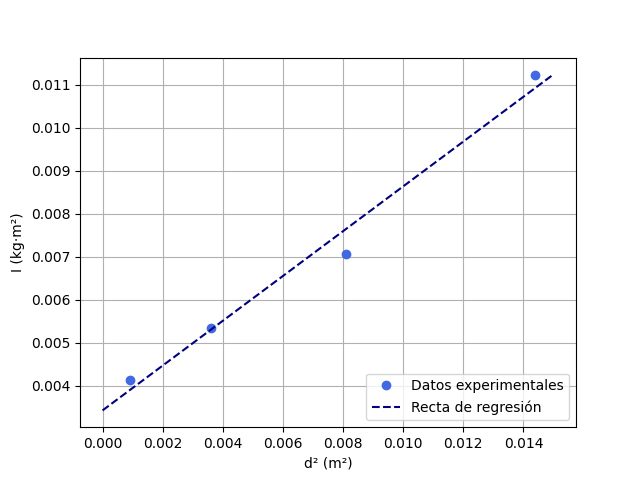
\includegraphics[width=0.85\linewidth]{Images/regSteiner1.png}
    \caption{Datos experimentales y regresión lineal del disco}
\end{figure}

A partir de los datos obtenidos en el ajuste podemos calcular el valor experimental de la masa del disco:

\begin{equation}
    m = 0.521 \pm 0.048 \; kg
\end{equation}

Si comparamos este valor con el medido directamente $(381,39 \;g)$ con la balanza podemos ver una clara diferencia. Esta diferencia puede tener explicaciones muy diversas, podría deberse a algún fallo experimental, a la falta de precisión en el ajuste que nos habría otorgado una regresión ponderada o a fallos en el cálculo. No obstante, el motivo que creemos que es culpable de la discordancia entre los valores es la falta de homogeneidad en los cuerpos. Siendo más concretos, cuando aplicamos el teorema de Steiner para hacer el ajuste estamos suponiendo que los cuerpos son ideales, homogéneos y con densidad constante. Este no es para nada nuestro caso, el disco se encontraba perforado y no se trataba de un disco ideal, cualquier heterogeneidad en su composición podría haber provocado esta diferencia.

\par Otra forma de verificar la precisión de nuestro análisis es comparando el valor obtenido del término independiente ($I_0$) con el valor teórico, calculado anteriormente y que resulta ser de $0,004262 \; kg \cdot m^2$. El valor obtenido en el ajuste fue de $0,003425 \; kg \cdot m^2$, que difiere bastante del valor teórico. Esta falta de precisión en el ajuste es otra de las posibles explicaciones de la falta de precisión en el cálculo de la masa del disco.

\subsubsection{Barra rígida}

En el siguiente apartado vamos a tratar de verificar el teorema de Steiner en otro cuerpo diferente, una barra rígida de $65,7 \; cm$ de longitud y $121,43 \; g$ de masa. Como explicaremos en la metodología vamos a tomar medidas para 10 valores de $d$, en concreto tomamos solo alrededor de 5 medidas del semiperíodo para cada valor de la distancia por problemas con el material.Los valores de $d$ para los que tomamos medidas con su incertidumbre son:

\begin{equation}
    d = n\cdot 1,0 \pm 0,1 \; cm \quad n = 1,2,3,...,10
\end{equation}

En las siguientes tablas representaremos los datos experimentales medidos en el laboratorio, incluyendo el momento de inercia en el propio centro de masas ($d=0$):

\begin{table}[h!]
    \centering
    \begin{tabular}{|c|c|c|c|c|c|c|}
    \hline
    $T_{1/2} \; (s)$ & $d=0 \;cm$& $d=1 \;cm$ & $d=2 \;cm$ & $d=3 \;cm$ & $d=4 \;cm$ & $d=5 \;cm$ \\ \hline
    1 & 1,595 & 1,606 & 1,625 & 1,649 & 1,689 & 1,681 \\ \hline
    2 & 1,596 & 1,606 & 1,633 & 1,643 & 1,686 & 1,688 \\ \hline
    3 & 1,595 & 1,606 & 1,627 & 1,648 & 1,677 & 1,681 \\ \hline
    4 & 1,600   & 1,607 & 1,629 & 1,651 & 1,685 & 1,682 \\ \hline
    5 & 1,595 &       & 1,632 & 1,646 & 1,671 & 1,680  \\ \hline
    6 & 1,596 &       &       & 1,661 &       &       \\ \hline
    7 & 1,561 &       &       &       &       &       \\ \hline
    \end{tabular}
    \caption{Datos del semiperíodo medidos en la bara para $d=[0;5] \; cm$}
    \label{Datos barra 1}
\end{table}

\begin{table}[h!]
    \centering
    \begin{tabular}{|c|c|c|c|c|c|}
    \hline
    $T_{1/2} \; (s)$ & $d=6 \;cm$& $d=7 \;cm$ & $d=8 \;cm$ & $d=9 \;cm$ & $d=10 \;cm$ \\ \hline
    1 & 1,697 & 1,738 & 1,772 & 1,826 & 1,866 \\ \hline
    2 & 1,71  & 1,732 & 1,785 & 1,829 & 1,871 \\ \hline
    3 & 1,703 & 1,738 & 1,782 & 1,833 & 1,876 \\ \hline
    4 & 1,700   & 1,732 & 1,781 & 1,831 & 1,879 \\ \hline
    5 & 1,703 & 1,729 & 1,777 & 1,825 & 1,87  \\ \hline
    6 &       & 1,724 &       &       &       \\ \hline
    \end{tabular}
    \caption{Datos del semiperíodo de la barra para $d=[6;10] \;cm$}
    \label{Datos barra 2}
\end{table}

\newpage

A partir de estos datos vamos a buscar un valor de referencia del semiperíodo para cada uno de los valores de $d$ y poder calcular así el momento de inercia aplicando la Ec.\ref{Calculo MI figuras}. Para buscar nuestro valor de referencia de $T_{1/2}$ vamos a aplicar un tratamiento estadístico similar al que llevamos aplicando durante toda la práctica. Por simplicidad vamos a representar en la siguiente tabla los datos inferidos de la muestra a partir de nuestro tratamiento. Los valores representados serán los valores finales, despúes de descartar las medidas que no entrasen en el intervalo de confianza. No obstante, los datos descartados serán comentados específicamente a continuación:

\begin{table}[h!]
    \centering
    \begin{tabular}{|c|c|c|c|c|c|}
    \hline
    $d \; (cm)$ & $\overline{T}_{1/2} \; (s)$ & Intervalo ($\overline{x}\pm 2\cdot s_A(x)$) & $s_A(T_{1/2}) \; (s)$ & $s_A(\overline{T}_{1/2}) \; (s)$ & $s_C(\overline{T}_{1/2}) \; (s)$  \\ \hline
    0  & 1,5962 & $[1,567;1,615]$     & 0,0018  & 0,00072 & 0,0012 \\ \hline
    1  & 1,6063 & $[1,60164;1,60336]$ & 0,00043 & 0,00022 & 0,001  \\ \hline
    2  & 1,6292 & $[1,6232;1,6352]$   & 0,003   & 0,0013  & 0,0017 \\ \hline
    3  & 1,6474 & $[1,6385;1,6609]$   & 0,0027  & 0,0012  & 0,0016 \\ \hline
    4  & 1,6816 & $[1,6684;1,6948]$   & 0,0066  & 0,003   & 0,0031 \\ \hline
    5  & 1,6824 & $[1,6767;1,6881]$   & 0,0029  & 0,0013  & 0,0016 \\ \hline
    6  & 1,7026 & $[1,6940;1,7112]$   & 0,0043  & 0,0019  & 0,0022 \\ \hline
    7  & 1,7322 & $[1,7223;1,7420]$   & 0,0049  & 0,002   & 0,0022 \\ \hline
    8  & 1,7794 & $[1,77045;1,7784]$  & 0,0045  & 0,002   & 0,0022 \\ \hline
    9  & 1,8288 & $[1,8228;1,8348]$   & 0,003   & 0,0013  & 0,0017 \\ \hline
    10 & 1,8724 & $[1,8632;1,8816]$   & 0,0046  & 0,0021  & 0,0023 \\ \hline
    \end{tabular}
    \caption{Datos obtenidos del análisis estadístico}
    \label{a}
    \end{table}


De entre todos los conjuntos de datos solo tuvimos que descartar dos valores, el valor de $1,561 \; s$ en los datos de $d=0$ y el valor de $1.661 \; s$ en los datos de $d=3 \; cm$. La media y la desviación típica ($s_A(T_{1/2})$) que figuran en la tabla son los valores obtenidos después de descartar esos datos y recalcular esos valores.

\newpage

\par A partir de estos datos vamos a calcular el momento de inercia y su incertidumbre para cada valor de $d$, que representaremos en la siguiente tabla acompañados de los valores de $d^2$ con los que realizaremos el ajuste. El ajuste realizado será igual que en el apartado anterior, de $I$ frente a $d^2$, donde el valor del momento para $d=0$ (El momento de inercia en el centro de masas) será el término independiente:

\begin{table}[h!]
    \centering
    \begin{tabular}{|c|c|c|c|c|}
    \hline
    $d \; (m)$ & $d^2\; (m)$ & $s(d^2) \; (m)$ & $I\;(kg\cdot m^2)$& $s(I)\;(kg\cdot m^2)$ \\ \hline
    0,010 & 0,000100 & 0,000020 & 0,00485 & 0,00046 \\ \hline
    0,020 & 0,000400 & 0,000040 & 0,00499 & 0,00047 \\ \hline
    0,030 & 0,000900 & 0,000060 & 0,00511 & 0,00048 \\ \hline
    0,040 & 0,001600 & 0,000080 & 0,00532 & 0,0005  \\ \hline
    0,050 & 0,00250 & 0,00010  & 0,00533 & 0,0005  \\ \hline
    0,060 & 0,00360 & 0,00012 & 0,00545 & 0,00051 \\ \hline
    0,070 & 0,00490 & 0,00014 & 0,00565 & 0,00053 \\ \hline
    0,080 & 0,00640 & 0,00016 & 0,00596 & 0,00056 \\ \hline
    0,090 & 0,00810 & 0,00018 & 0,00629 & 0,00059 \\ \hline
    0,100  & 0,01000 & 0,00020  & 0,00660  & 0,00062 \\ \hline
    \end{tabular}
    \caption{Datos de los momentos de inercia empleados en el ajuste}
    \label{Datos steiner 2}
\end{table}


Donde $s(d^2)$ viene dada, al igual que en el apartado anterior, por esta expresión:

\begin{equation}
    s(d^2) = 2d \cdot s(d)
\end{equation}

En este caso el valor de $s(d)$ viene dado por la precisión instrumental de la regla, $0,001 \;m$.

\par A partir de estos datos realizamos la regresión lineal simple con término independiente, donde obtuvimos los siguientes valores para nuestra recta (Del tipo $y=a+bx$):

\begin{equation}
    \begin{gathered}
        a = 0.004893 \; kg \cdot m^2 \\
        b = 0.1693 \; kg \\
        s(a) = 3.3\cdot 10^{-5} kg \cdot m^2 \\
        s(b) = 0.0070 \; kg \\
        s = 7.6 \cdot 10^{-5} \\
        r = 0.992
    \end{gathered}
\end{equation}

Por tanto, en aplicación del teorema de Steiner, la masa de la barra metálica es de:

\begin{equation}
    m = 0.1693 \pm 0.0070 \; kg
\end{equation}

En cuánto al término independiente debemos notar que corresponde con el valor de $I_0$ respecto al centro de masas. Otra forma de verificar la exactitud de nuestro ajuste es calcular el valor teórico de ese momento de inercia con su incertidumbre, a partir de la Ec.\ref{MI cuerpos geometricos} y de la Ec.\ref{Inc MI figuras}:

\begin{equation}
    I_0 = 0.004368 \pm 1,3 \cdot 10^{-5} \; kg \cdot m^2
\end{equation}

El valor obtenido en el ajuste para el término independiente ($I_0$) es de $0,004893 \; kg\cdot m^2$, próximo al teórico, por lo que podemos concluir que nuestro ajuste es fiel a la realidad, pese a no emplear el ajuste ponderado.

En la siguiente gráfica podemos ver representado nuestro ajuste por mínimos cuadrados, además de los valores experimentales:

\begin{figure}[h!]
    \centering
    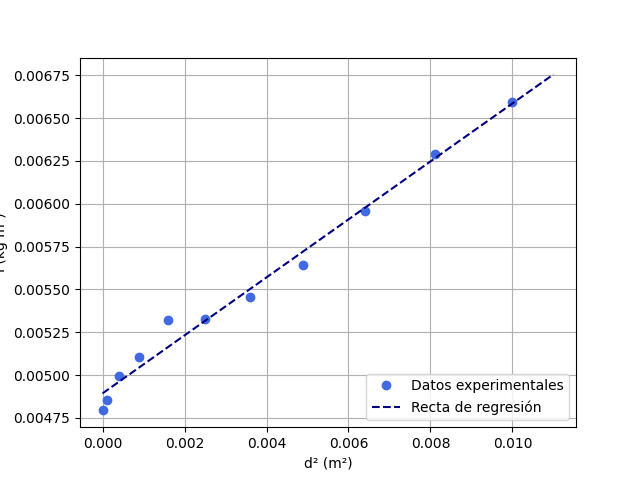
\includegraphics[width=0.75\linewidth]{Images/regSteiner2.png}
    \caption{Datos experimentales y regresión lineal de la barra metálica}
\end{figure}

\newpage

\section{Conclusiones}

Esta práctica se centró en dos pilares fundamentales, el cálculo del momento de inercia de diferentes cuerpos y la verificación del teorema de Steiner. En la primera parte de la práctica obtuvimos los siguientes resultados de valores experimentales y teóricos para el momento de inercia de los tres cuerpos:

\begin{table}[h!]
    \centering
    \begin{tabular}{|c|c|c|}
        \hline
        Cuerpo & $I_E \pm s(I_E) \; (kg \cdot m^2)$ & $I_T \pm s(I_T) \; (kg \cdot m^2)$  \\ \hline
        Disco &$0.003847 \pm 4.9 \cdot 10^{-5}$ & $0.004262 \pm 0.000074$ \\ \hline
        Cilindro & $0.0003557 \pm 4.8 \cdot 10^{-6}$ & $0.00048036 \pm 0.00000025$ \\ \hline 
        Esfera & $0.000997 \pm  1,3 \cdot 10^{-5}$ & $0.000726 \pm 0,000045$ \\ \hline
    \end{tabular}
    \caption{Resultados experimentales y teóricos de los momentos de inercia}
\end{table}

Como podemos ver los resultados obtenidos, aunque no entran dentro del rango de incertidumbre, están bastante cerca de los valores teóricos. Estas pequeñas discordancias pueden tener muchos orígenes, pero el principal es probable que sea que no estamos trabajando con cuerpos ideales, como supone la fórmula que empleamos para calcular el momento teórico. Pese a todo los resultados experimentales podemos concluir que son bastante satisfactorios.

\par Por otro lado, la segunda parte de la práctica trató de verificar el teorema de Steiner. La forma de verificarlo fue comprobar si la masa de los cuerpos con los que trabajamos coincidía con la pendiente de nuestra recta de regresión, como explicamos más detalladamente durante la práctica. Los resultados obtenidos fueron:

\begin{table}[h!]
    \centering
    \begin{tabular}{|c|c|c|}
        \hline
        Cuerpo & $m \pm s(m) \; (kg)$ & $m_E \pm s(m_E) \; (kg)$ \\ \hline
        Disco & $0,38139 \pm 0.00001$ & $0.521 \pm 0.048$ \\ \hline
        Barra & $0,12143 \pm 0,00001$ & $0.1693 \pm 0.0070$ \\ \hline
    \end{tabular}
    \caption{Resultados experimentales obtenidos en la segunda parte}
\end{table}

siendo $m$ la masa medida directamente con la balanza y $m_E$ el valor de la masa obtenido con el ajuste. Igual que en el apartado anterior los resultados difieren del valor real, aunque se observa cierta coherencia en las medidas. En esta parte de la práctica la causa de ese error en las medidas se debe probablemente al material empleado, en concreto al resorte, que provocó grandes problemas a la hora de tomar las medidas. Estos problemas fueron los que provocaron que no pudiéramos obtener una muestra suficientemente grande de medidas, otra de las posibles causas de la falta de precisión.

\par Finalmente, podemos concluír que, pese a los problemas sufridos, conseguimos alcanzar los objetivos propuestos en esta práctica, además de haber profundizado en gran medida en el concepto de momento de inercia y en su relación con las magnitudes que caracterizan un movimiento oscilatorio.

\end{document}